\documentclass{sigchi}

% Use this command to override the default ACM copyright statement (e.g. for preprints).
% Consult the conference website for the camera-ready copyright statement.


%% EXAMPLE BEGIN -- HOW TO OVERRIDE THE DEFAULT COPYRIGHT STRIP -- (July 22, 2013 - Paul Baumann)
% \toappear{Permission to make digital or hard copies of all or part of this work for personal or classroom use is 	granted without fee provided that copies are not made or distributed for profit or commercial advantage and that copies bear this notice and the full citation on the first page. Copyrights for components of this work owned by others than ACM must be honored. Abstracting with credit is permitted. To copy otherwise, or republish, to post on servers or to redistribute to lists, requires prior specific permission and/or a fee. Request permissions from permissions@acm.org. \\
% {\emph{CHI'14}}, April 26--May 1, 2014, Toronto, Canada. \\
% Copyright \copyright~2014 ACM ISBN/14/04...\$15.00. \\
% DOI string from ACM form confirmation}
%% EXAMPLE END -- HOW TO OVERRIDE THE DEFAULT COPYRIGHT STRIP -- (July 22, 2013 - Paul Baumann)


% Arabic page numbers for submission.
% Remove this line to eliminate page numbers for the camera ready copy
% \pagenumbering{arabic}


% Load basic packages
\usepackage{balance}  % to better equalize the last page
\usepackage{graphics} % for EPS, load graphicx instead
\usepackage{times}    % comment if you want LaTeX's default font
\usepackage{url}      % llt: nicely formatted URLs

\usepackage{multirow}
\usepackage{ wasysym }
\usepackage{ textcomp }
\usepackage{tabularx}
\usepackage{mathtools}
\usepackage[valuemode=math,unitmode=math]{siunitx}


% llt: Define a global style for URLs, rather that the default one
\makeatletter
\def\url@leostyle{%
  \@ifundefined{selectfont}{\def\UrlFont{\sf}}{\def\UrlFont{\small\bf\ttfamily}}}
\makeatother
\urlstyle{leo}


% To make various LaTeX processors do the right thing with page size.
\def\pprw{8.5in}
\def\pprh{11in}
\special{papersize=\pprw,\pprh}
\setlength{\paperwidth}{\pprw}
\setlength{\paperheight}{\pprh}
\setlength{\pdfpagewidth}{\pprw}
\setlength{\pdfpageheight}{\pprh}

% Make sure hyperref comes last of your loaded packages,
% to give it a fighting chance of not being over-written,
% since its job is to redefine many LaTeX commands.
\usepackage[pdftex]{hyperref}
\hypersetup{
pdftitle={Aesthetic Electronics: Designing, Sketching, and Fabricating through Digital Exploration},
% pdftitle={Ellustrate: Designing, Sketching, and Fabricating Aesthetic Electronics through Digital Exploration},
pdfauthor={LaTeX},
pdfkeywords={SIGCHI, proceedings, archival format},
bookmarksnumbered,
pdfstartview={FitH},
colorlinks,
citecolor=black,
filecolor=black,
linkcolor=black,
urlcolor=black,
breaklinks=true,
}

% create a shortcut to typeset table headings
\newcommand\tabhead[1]{\small\textbf{#1}}

% set up tight list spacing
\usepackage{enumitem} 
\setlist{nolistsep,nosep}

% for toggles
\usepackage{etoolbox}


% CHANGE FROM TOGGLE TRUE TO TOGGLE FALSE TO HIDE COMMENTS
\newtoggle{comments}
\toggletrue{comments}
% \togglefalse{comments}

% Comment region command (from Wesley Willett)
\usepackage[usenames]{color}
\usepackage[usenames,dvipsnames]{xcolor}
\iftoggle{comments} {
  %if we want to show comments
  \newcommand {\jlo}[1]{{\color{magenta}\bf{JLO: #1}\normalfont}}
  \newcommand {\cesar}[1]{{\color{NavyBlue}\bf{CAT: #1}\normalfont}}
  \newcommand {\ep}[1]{{\color{violet}\bf{EP: #1}\normalfont}}
  \newcommand {\mira}[1]{{\color{Orange}\bf{MD: #1}\normalfont}}
  \newcommand {\wil}[1]{{\color{Blue}\bf{WL: #1}\normalfont}}
  \newcommand {\danny}[1]{{\color{Red}\bf{DK: #1}\normalfont}}
}{
  %if we don't want to show comments
  \newcommand {\jlo}[1]{}
  \newcommand {\cesar}[1]{}
  \newcommand {\ep}[1]{}
  \newcommand {\mira}[1]{}
  \newcommand {\wil}[1]{}
  \newcommand {\danny}[1]{}
}

\newenvironment{myquote}{\list{}{\leftmargin=0.01\textwidth \rightmargin=0.01\textwidth}\item[]}{\endlist}
\newcommand*{\quoted}[1]{{\small{\fontfamily{cmss}\selectfont{#1}}}}
\newcommand*{\layer}[1]{{\textbf{\small{\fontfamily{cmss}\selectfont{#1}}}}}
\newcommand*{\participant}[1]{{\textbf{\small{\fontfamily{cmss}\selectfont{#1}}}}}
\newcommand*{\factor}[1]{{\textbf{\small{\fontfamily{cmss}\selectfont{#1}}}}}
\newcommand*{\nt}[1]{{\textbf{\small{\fontfamily{cmss}\selectfont{#1}}}}}
\newcommand*{\code}[1]{{\small{\fontfamily{cmss}\selectfont{#1}}}}




% End of preamble. Here it comes the document.
\begin{document}

\title{Aesthetic Electronics: Designing, Sketching, and Fabricating through Digital Exploration}
% \title{Ellustrate: Designing, Sketching, and Fabricating Aesthetic Electronics through Digital Exploration}

% \title{Ellustrate: Enabling Aesthetic Design and Fabrication for Silver, Copper, and Conductive Thread Circuits}
% \title{Ellustrate: Enabling Visual Circuit Design and Fabrication for Multiple Materials}

\numberofauthors{1}
\author{
  \alignauthor Anonymized for Submission\\
    \affaddr{...}\\
    \affaddr{...}\\
    \email{...}
}
\teaser{
  \vspace{-20pt}
  \centering
  \includegraphics[width=\linewidth]{figures/teaser.pdf}
  \caption{
    Sketched digital circuits (top), and fabricated circuits (bottom) created through various craft mediums: a) copper tape painting on paper, b) sewn conductive thread on fabric, c) painted graphite ink as interative illustration, and d) decorative silver ink to ornament physical objects.
  }
    \vspace{-8pt}
  \label{fig:teaser}
}

\maketitle

\begin{abstract}
As interactive electronics become more intimate and personal, the design of the circuitry has developed a more playful and creative aesthetic as well. Circuit sketching and design is a multidimensional activity combining the arts, crafts, and engineering, and broadens participation of electronic creation to include makers of diverse backgrounds. In order to support this design ecology, we present Ellustrate, a digital design tool that enables the functional and aesthetic design of electronic circuits with multiple conductive and dielectric materials. Ellustrate guides users through fabrication and debugging process, easing the task of practical circuit creation while supporting designers' aesthetic decisions throughout circuit authoring workflow. In a formal user study, we demonstrate how Ellustrate enables a new electronic design conversation that combines electronics, materials, and visual aesthetic considerations. 

% Circuit sketching has gained traction in creative communities as a method of democratizing circuit creation, diversifying the materials and techniques used to make unique, critical artifacts. In order to support this design ecology, we present Ellustrate, a digital design tool that enables the functional and aesthetic design and fabrication of electronic circuits.
% Ellustrate incorporates a holistic design cycle in a digital design tool which guides users through all essential steps towards realizing their electronic ideas. The tool provides designers with a digital assistive artboard which aids users with constructing electrically-valid circuits through a set of visual rules. Using a connectivity graph, we can provide step-by-step material-specific fabrication and debugging instructions for each design.
% In a formal user study, we show how Ellustrate enables a new circuit aesthetic that operates beyond efficiency, and can serve as a scaffold for designers and artists to incorporate electronic design in their everyday practice.
% We discuss how such tools that enable material-first exploration can support growing online communities. 


% and incorporates story-telling and new mental model.

% democratize electronic design to include designers and artists and examine the aesthetic value of circuit design beyond
% Ellustrate provides multi-material support and design-focused drawing tools tailored for aesthetically-driven functional circuit design. 
% Within the Ellustrate design tool, designers receive immediately feedback and corrections on their circuit design as they create their electronic artwork.
% Beyond the electrical and visual design, Ellustrate also offers step-by-step guidance on fabricating and debugging.

\end{abstract}
\keywords{
	design tool; sketching circuits; fabrication  \newline
}

\category{H.5.m.}{Information Interfaces and Presentation (e.g. HCI)}{Miscellaneous}

\section{Introduction}
The landscape of electronics is rapidly changing. Devices are becoming exponentially smaller, requiring electronic circuits to be printed directly on the device housing and on ultra-thin wearables~\cite{MacDonald:2014ju,Kim:2014iq}. As such, new designs must blend functional and structural design variables. Echoing the Radical Atoms vision, such designs compel ``new material design principles'' to be created that ``treat objects as homogeneous entities with the ability to change their properties''~\cite{Ishii:2012fg}.

In this paper, we introduce the term \textit{Aesthetic Electronics} to describe a class of electronics that foregrounds both functional electronics and visual aesthetics interrelated design variables. In such electronics, design principles (e.g. form and symmetry) affect how designers choose materials and make marks; in tandem, these choices affect electrical design variables (e.g. resistance, capacitance, and inductance). In practice, Aesthetic Electronics can enhance the making experience to engage various crafting and art practices and contextualize circuit designs (Figure \ref{fig:teaser}).
\begin{figure*}[ht]
 \vspace{-16pt}
\centering
  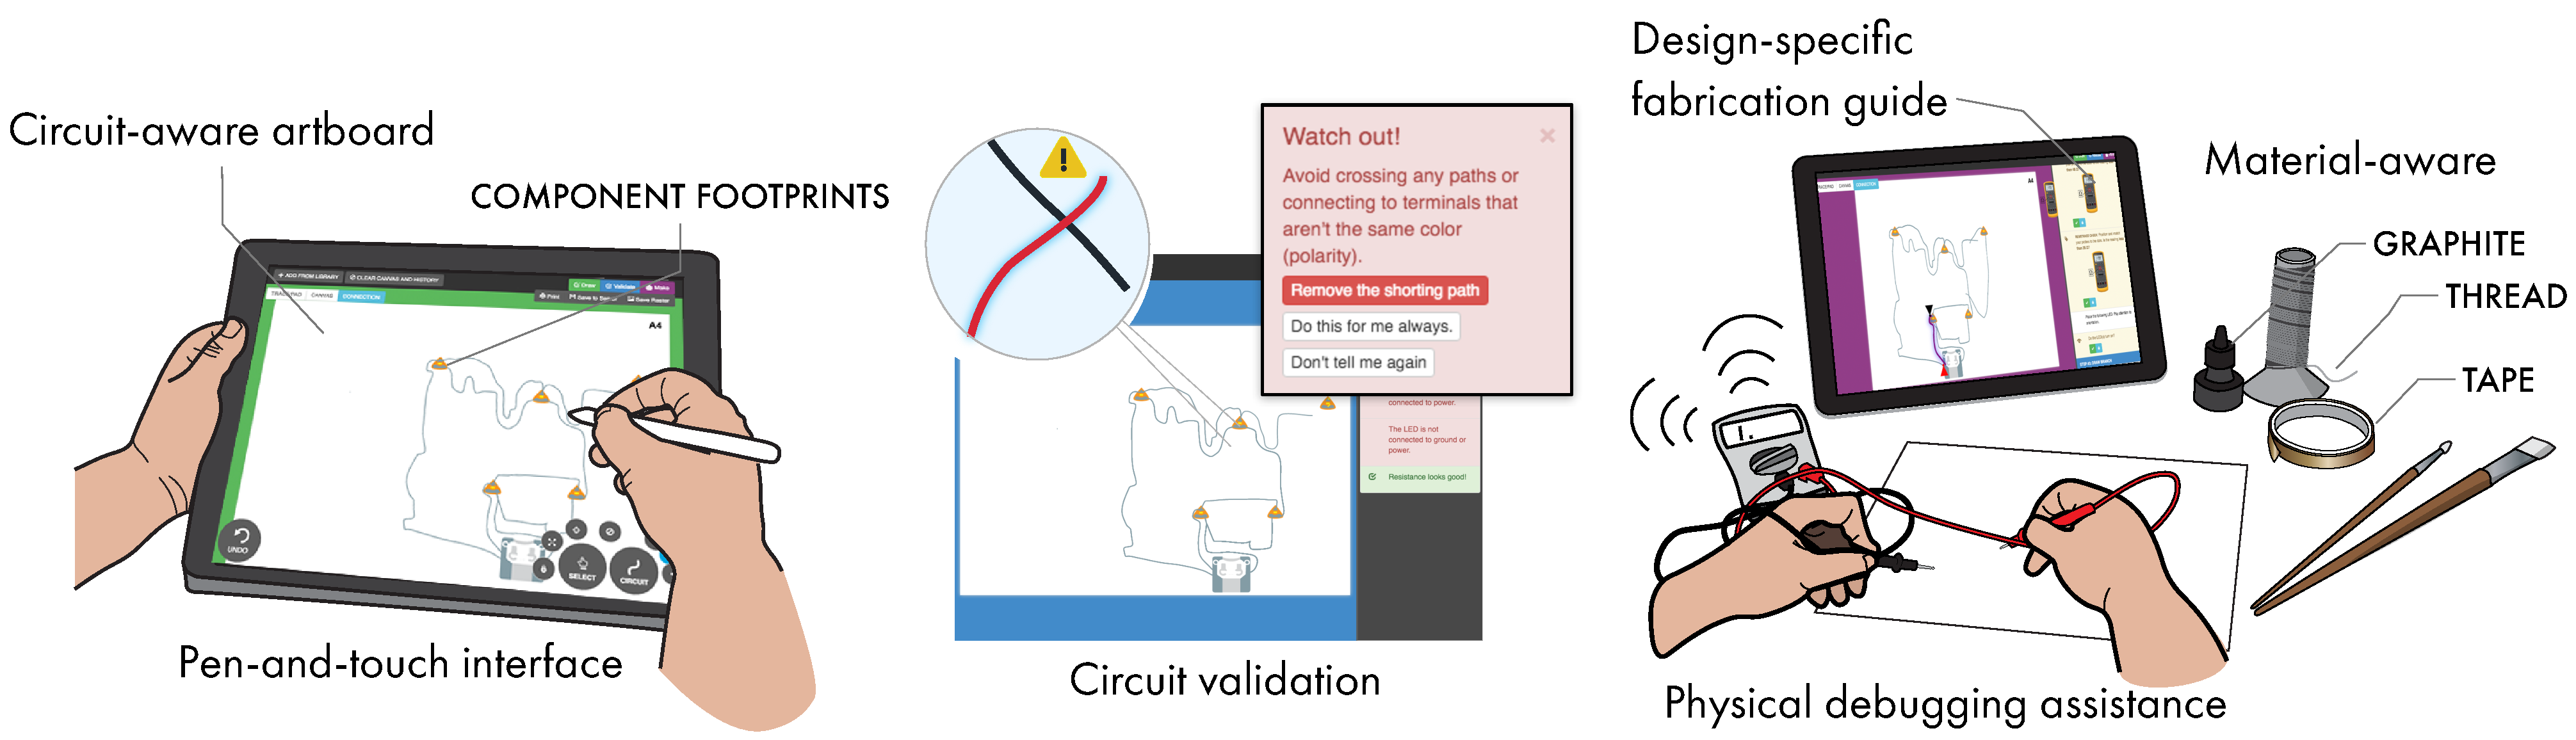
\includegraphics[width=\linewidth]{figures/ellustrate_system.pdf}
  \caption{Ellustrate circuit creation process. The user sketches a digital design on a circuit-aware artboard. The tool validates the circuit and the user corrects electrical errors if necessary. Custom fabrication instructions are produced to guide the user in making a physical circuit.}~\label{fig:process_flow}
  \vspace{-16pt}
\end{figure*}

This work focuses on the creation of a subset of Aesthetic Electronics - \textit{Aesthetic Circuits} which explores electrical traces as a site of creativity.
Contrasted with the broader field of Aesthetic Electronics, where active physical devices (i.e. capacitors, strain gauges, speakers) can be made with aesthetic value, Aesthetic Circuits focuses on the design of the passive electrical traces. 
Traces are currently one of the most restricted design element in circuit design tools, resulting in circuit layouts with rectilinear, efficiency-focused designs.
Even in design tools that focus on entry-level circuit making, such as 123D Circuits and Fritzing, the functions for drawing the final printed circuit board layout still favor the traditional straight-line aesthetic~\cite{_autodesk123d_????}.
While this tried-and-true layout method is extremely valuable, it also limits how electronics and circuits are viewed as something pedantic instead of creative. Despite the tremendous benefits brought to electronic circuit creation, these tools and processes have remained restricted to a physical classroom setting ~\cite{qi_stickers_2015,qi_sketching_2014}.   
    


Creating Aesthetic Electronic designs requires a unique fluency over the affordances and electrical properties of materials.
We enable Aesthetic Circuit design through Ellustrate, our digital design and fabrication asssitance tool (Figure \ref{fig:process_flow}). Ellustrate, leverages a process known as ``sketching circuits", a design and fabrication process that enables the creation of physical circuit with craft materials~\cite{qi_sketching_2014}. As a natural and intuitive process, sketching is a shared skill amongst professional engineers, designers, makers and artists. Moreover, the circuit sketching process has shown to be increase participation of electronic design from diverse population, remove negative stigma associated with circuits, and motivate early learners~\cite{qi_stickers_2015}. Various research fields have taken notice of the circuit sketching trend as well, creating various conductive materials (i.e silver, graphite, copper) that can be applied on paper in ways similar to a regular pen~\cite{russo2011pen,Anonymous:ojhPyGTN}. We see supporting Aesthetic Circuit sketching as a step towards broadening the definition of electronic design and altering the narrative of who participates in circuit making. 

While the usability of conductive materials has enabled many creative crafting projects, we believe the complexity and creativity in electronic craft can be further augmented by providing two critical elements -- a digital circuit-design sandbox and assistance for physical fabrication and debugging. Ellustrate provides a natural sketching interface on a tablet, electronic design validation, and fabrication and debugging guidance (Figure \ref{fig:process_flow}). 
%\ep{these are key parts of the contribution...you may want to put them much earlier or call them out as distinctly novel more prominently.}
Ellustrate differs from most circuit design tools in a number of ways summarized by Figure \ref{fig:comparison_table}: a) it balances concerns of electronic validity and expressive design, b) it integrates the human back into the fabrication process, shown in prior work to improve engagement with techniques and processes~\cite{anonmyzied_proxy}, and c) provides debugging assistance to aid users with correcting improperly fabricated circuits. We performed formative interviews, pilot studies, and formal user studies in order to accomplish these design goals. 


\begin{figure}[b]
\centering
  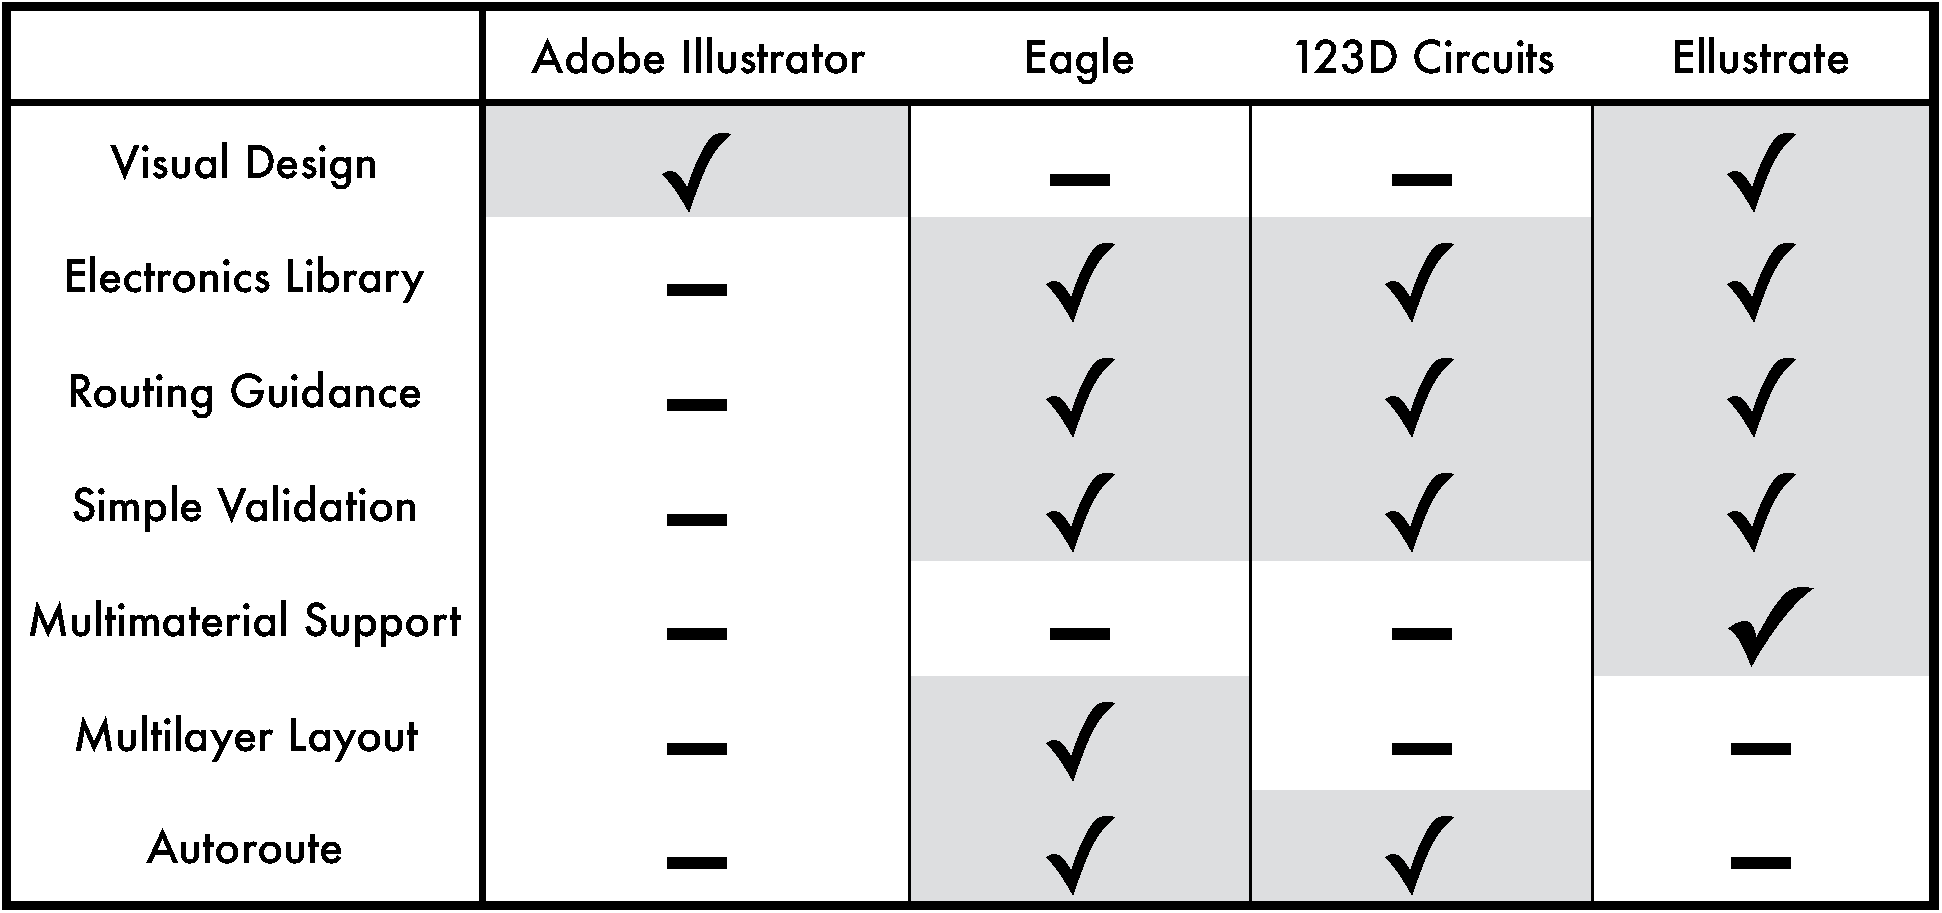
\includegraphics[width=1\columnwidth]{figures/comparative_table.pdf}
  \caption{A comparison of design tool features. Ellustrate provides coverage for both visual design and circuit design concerns. }~\label{fig:comparison_table}
  \vspace{-16pt}
\end{figure}

% \cesar{this is just rewriting the figure caption...}
% : for example, a painting can be augmented using LED stickers and copper tape (Figure \ref{fig:teaser}a), clothing can be decorated with a graphical circuit made with conductive thread (Figure \ref{fig:teaser}b), the narrative of a picture book can be enhanced with graphite paint illustrations (Figure \ref{fig:teaser}c), and the surface of a 3D box can be decorated with a silver ink circuit(Figure \ref{fig:teaser}d).
% in order to balance both functional and aesthetic requirements.

% aims to further democratize the electronic design process to include artists and designers with no prior circuit knowledge by 
% Sketching has shown to bring interesting elements to hardware prototyping, sparking creative innovations within the Maker community. 
% Although sketching circuit has many benefits in initial design and early electronic education, it is not explored by supported by many electrical digital design tools.
% Drawing and sketching play a critical role within the development of user interfaces. 
%The traditional circuit design aesthetic is mostly influenced by efficiency - how to pack as many lines as possible in shortest distance from one component to another. This is an artifact of the huge demand on miniaturization of electronics and the exponentially increasing burden on electronics to conserve valuable board space. The industry-standardized interest in optimizing for speed and space have influenced early circuit education, even when optimized performance is not as big of a concern compared to eliciting interest and retaining learners.

% \jlo{Sketching is an integral part of design - in both visual design, and software and hardware engineering design. Digital design tools that aid in physical design have been studied extensively, and their benefits to the final physical design have been well documented. (notes to be flushed out: Material exploration - the ability to think of atoms and bits as clay - traces are not just automatic connections but of varying resistance and other properties - device physics thinking...)}
% As electronic devices become more intertwined and intimate with users, the internal making of them becomes more naked and transparent. Along with the advent of structural electronics, where circuit traces and components are printed on housing of an electronic device, and wearable electronics, where electronics and active components are part of the fashion aesthetics, the ability to inject visual design into functional electronics become increasing important.



\section{Related Work}
To create a digital tool that enables the physical creation of physical circuits, we based our work on established research on nontraditional circuits and electronics, as well as relevant digital tools. 
on ofa
\subsection{Sketching Electronics on Familiar Materials}
By fabricating electronics on a familiar material, like paper, users can explore electronic design using a previously held skill set.  Augmenting such common everyday materials with power, lights, and motions has been shown to introduce a sense of wonder that resonates with people of diverse ages and backgrounds~\cite{karagozler_paper_2013,Qi:2010tp,qi_stickers_2015,qi_sketching_2014} Crafting have shown to be a powerful technique in STEM education that encourages interdisplanary participations and further democratizes makeing and science education~\cite{qi_sketching_2014}.
Furthermore, the role of these materials in everyday life has been shown to be a natural platform for story-telling with electronics~\cite{Jacoby:2013cq}. As such, incorporating familiar materials in circuits has altered the design landscape leading to more natural, organic, and novel circuit layouts.
As more conductive and non-conductive materials develop, as does the complexity of understanding the unique electronic intricacies of each material~\cite{Hodges:2014cm}.  Ellustrate aims to support the circuit sketching practice by providing a digital design tool that provides support for working with different materials and encourages an aesthetic exploration of circuit designs.

% Qi et al. cited the expressive medium as the main reason for the successful recruitment of a diverse population who participated in the sketching circuit workshop.
% Buechley et al. and Qi et al. expanded upon the story-telling narrative of paper circuits by leveraging sketching on paper at the onset of the creative ideation. 
% By utilizing the familiarity of a regular pencil, sketching circuits was able to combine the ideation process for both circuit and art design under one platform. (reword).  \cesar{this is too over-reaching}
 % and complement the visual design of the work.



\subsection{Digital Sketching Tools} 
Since sketching is such an important element of early stage design, many digital tools have been created to facilitate this process. These tools transform sketches into prototypes of a final design by decomposing and recognizing domain-specific symbols and lines. In SILK and SATIN, Landay et al. and Hong et al. investigate a set of software support functions for sketching user interfaces, website design, and simple logic circuits~\cite{Hong:2007ta,Landay:1996wn}. The two tools generate a final design by ``cleaning up'' imperfections in the hand-drawn sketches -- short, overlapping lines are combined, strokes are straightened, and imperfect symbols of logic gates are corrected. The traces between the elements are often reduced to the the shortest straight path possible. With the goal of exploring the creative value in the sketches, Ellustrate does not correct or reduce the electrical traces (other than for electrical functional reasons). 


\subsection{Digital Design Tools for Physical Designs}
Digital tools have revolutionized the hardware prototyping process by allowing users to iterate on a digital design before creating the physical version through simulations of the electric and mechanical properties. Digital tools provide educational guidance for various aspects of the physical making process. In PaperPulse, users can program the behavior of a microcontroller, print out the design using a conductive ink printer, and fabricate the design with instructions generated by the tool~\cite{RafRamakers:2015gb}. In d.tools, designers can design and iterate hardware interactions using statecharts to control a microntroller and plug-and-play hardware (i.e. slider, LED)~\cite{hartmann_reflective_2006}. Within the AutoDesk CircuitScribe design tool, users can sketch and simulate circuit designs. The design can then be printed on a piece of paper and traced over with a silver pen~\cite{_autodesk_????}. Ellustrate expands upon the aforementioned work by 1) implementing a sketching platform for pen-and-tablet to emulate a more natural sketch interaction, 2) augmenting the avaliable electronic component footprints and materials library to support a diverse set of circuit components footprints, and 3) integrating fabrication and debugging guidance to lower the barrier of entry for users with little circuit background.


\section{Formative Interviews}
As much as these creative forms of circuits enable early exploration of the circuit design, there are a few areas that could be improved in order to facilitate creative exploration in circuit design. In order to articulate the common difficulties that users encounter in the early stage of circuit design, we performed a series of formative user studies and interviews. 

To learn about opportunities for supporting circuit sketching and fabrication with a digital design tool, we interviewed three circuit educators and seven potential users. 
Educators were experienced in teaching students with no prior electronic design knowledge from different domains: an introductory circuits Massive Open Online Course (MOOC), Maker Faire workshops, and circuit sketching workshops. 
Potential users recruited were university students with little to no circuits background, but with varying level of design experience. Utilizing a think-out-loud protocol, we asked four interviewees to design a circuit with two different colored markers to study possible visual styles, and three interviewees to design and fabricate three simple  LED\footnote{Chibitronics LED stickers} circuits with copper tape (eliciting help from the interviewer as needed) to study potential fabrication and debugging problems. We note two major observations that informed the design of our system.

\subsubsection{Immediate Feedback and Validation}
In hardware design, there are two main types of error that a user might encounter -- electronic design rule violations (i.e. electrical shorting), and functional errors (i.e. parallel LED's routed as series). They are closely analgous to the classifications of syntax and semantic errors in software. Digital tools are immensely useful when it comes to catching syntax errors within a circuit design, but there are few hardware design tools that provide design feedback in a way that is accessible to early learners. All experts we interviewed agreed that a electrical design check as immediate feedback during the design process would greatly benefit early learners. Their opinions were well-supported by exisitng literature -- according to ~\cite{Hattie:2007gi,Epstein:2002ur}, providing specific immediate feedback is crucial in early learning. Our circuit learners reported having more confidence in their subsequent design decisions if positive and negative feedback were given immediately, especailly in the beginning of the design process. Although Ellustrate is not structured as a tool specific for learning, it does aim to build lasting good electrical design habits. During the circuit sketching process, we observed that the design rule that most users have trouble with was keeping track of ground and power pads, and preventing attached traces from shorting out the circuit.

\subsubsection{Expert Knowledge and Guidance}
During our interviews, we quickly learned from our early circuit learners that the result of the fabrication step could be most rewarding if successful, but the most demoralizing and frustrating if not. Unfortunately, assistance in fabrication and circuit debugging are not provided in most circuit design tool, and instructions in this realm remain mostly restricted to in-person classroom/workshop setting~\cite{Klemmer:2004ul}. We feel that providing a debugging and fabrication guide is crucial to achieving our goal of empowering designers. One major difference in fabrication that we observed in experts and entry level circuit makers was the ability to modularize their circuits into small, individually-testable sections in a way that might minimize the chances of error propagation. We formulated expert advice into rational steps that users can follow to fabricate their design. Furthermore, experts articulated the need for in-situ debugging advice or else risk potentially overloading a learner with too much information. 

% More detailed and in-depth information and debugging suggestions can be accessed as desired by the user.  
% the benefits of templates/examples in the early learning process of non-experts
% static template and their potential shortcoming 
% cite related step-by-step design tool work 


\begin{figure}
\centering
  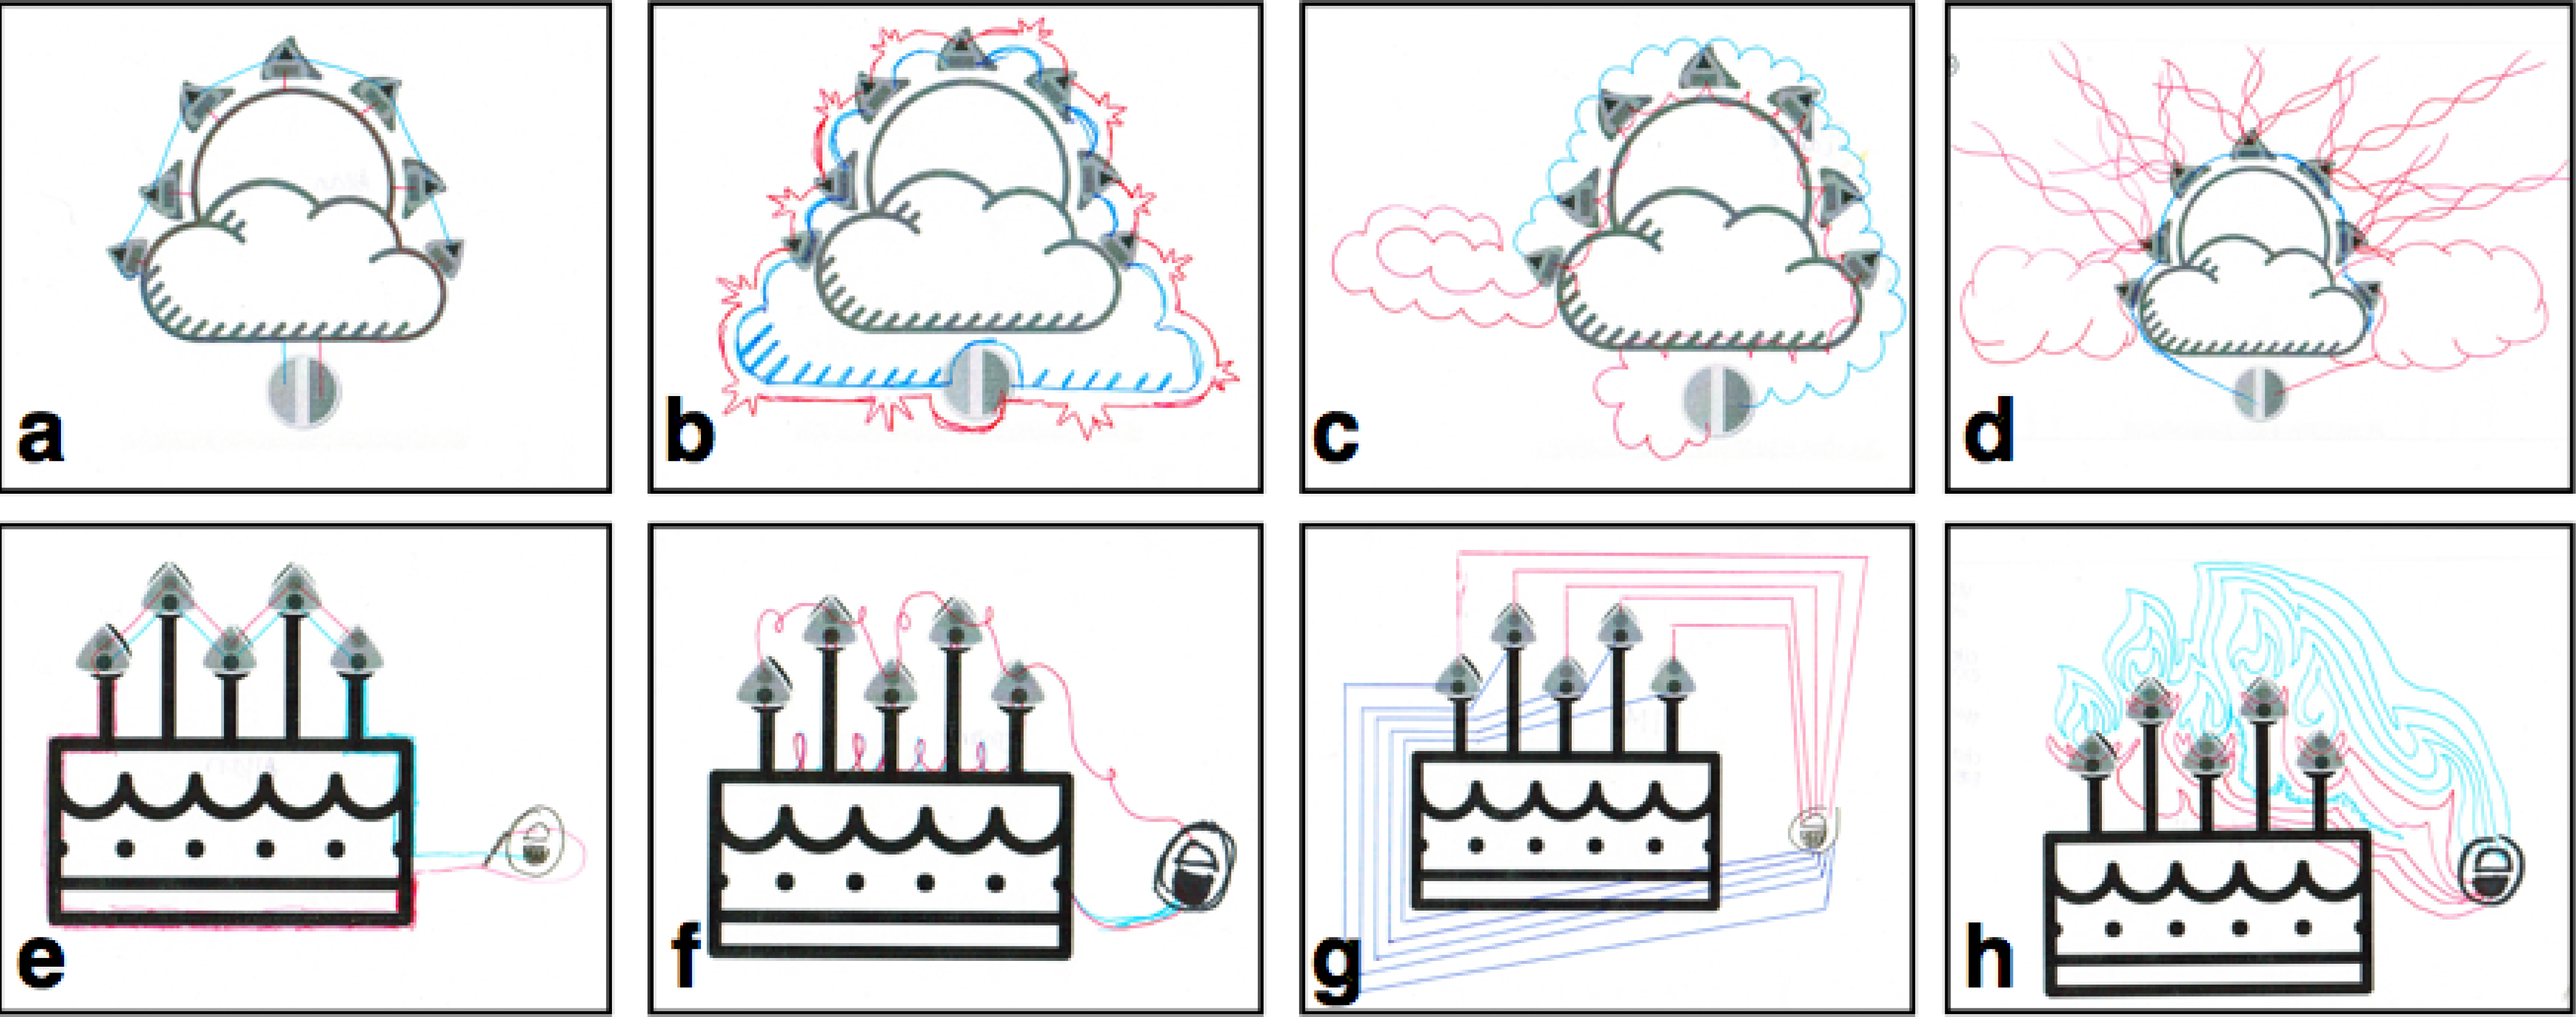
\includegraphics[width=1\columnwidth]{figures/Ellustrate_figures_formative_user_design}
  \caption{Circuit designs from the formative study drawn with non-conductive ink pens on paper. Red lines represent power and blue line represent ground. With either a sun and clouds (a-d) or a birthday cake (e-h) as an artistic scaffold, the complexity of the interviewees' circuits varied considerably }~\label{fig:formative_user_design}
  \vspace{-16pt}
\end{figure}

% \section{Critical Elements for an Aesthetic Circuit Design Tool}
\section{Aesthetic Circuit Design Objectives}
The design of Aesthetic Circuits faces key challenges due to the careful considerations and balance of electrical, material, and visual design principles. There are four major features that a digital tool for aesthetic tool needs to include: 

\subsection{Freeform Circuit Drawing Tool}
The design of electrical traces that possess both electrical function and aesthetic properties is possibily the most critical task in creating Aesthetic Circuits. In traditional circuit design tools, routing assistance is done in the form of auto trace -- a algorithm-driven process that determines the shortest and most efficient paths to connect electronic components on a given circuit board~\cite{Fisk:1965tk}. Autotrace creates routing that minimizes board space and noise, but does not provide any aesthetic freedom. On the other hand, the design of Aesthetic Circuits, although still retaining the need for functionality, has less of a concern in minimizing board space and noise. Therefore, a digital tool for Aesthetic Circuit design needs to provide the freedom of creating artistic drawing but provide enough restrains to simultaneously ensure electrical function. Just as breadboarding results in ``wire nests", sketching circuits can quickly become a complex circuit routing puzzle especially when combined with visual design.
When the electronic components are placed in a nonlinear fashion, powering all of them without shorting the circuit or creating excessively long traces become difficult. In Qi el al, a paper template is provided to workshop participants to guide them in placing copper tape~\cite{Qi:2014bg}. While this method is highly effective in aiding participants in creating functional circuits, it limits creativity in visual design ~\cite{Qi:2014bg}. Within Ellustrate, users are encouraged to explore and iterate different placements of electronics components and traces to optimize the balance between visual design and circuit functionality. 
%\ep{figure 4 shows teh creative diversity for routing (but not placement)}

\subsection{Electronics and Materials Library}
Footprint and electronic properties (i.e. turn on voltage, maximum current) are important criteria in any circuit design. The understanding of these properties is essential to creating visually pleasing and functional circuit design. However, this vital information, which is readily available in any circuit design software (i.e. Eagle, Cadence, 123D Circuits), are not provided in any visual design software. This greatly limits the ability of the designer to create a functional circuit while exploring the visual elements of an electronic component footprint. In addition to the lack of electronic libraries, users that create physical circuits with nontraditional materials such as silver paint, graphite, and conductive thread face aditional difficulties fabricating traces with varying, uncharacterized, and relatively high resistive materials (compared to the traditional copper traces). These long, highly resistive traces often cause problems that are invisible to designers with little circuit design experience~\cite{admin:2009wf}. 

\subsection{Fabrication and Debugging Guidance}
  The physical fabrication of the designed circuit is a difficult step in the creative process, as discovered in the Qi et al study, our expert survey, and formative user study. Solving hardware problems, which often requires probing to locate the issue, can seem like a ``dark art" to early circuit learners and heavily relies on tacit knowledge. In a workshop setting, guidance is provided to the participants to fabricate the circuit and debug any problems~\cite{qi_sketching_2014}. However, in-person guidance is not easily scalable. Within Ellustrate, fabrication steps are provided in a step-by-step guideline, incorporating the modular fabrication process recommended by experts, where as debugging guidance is provided in an expandable menu for users to access as needed. 

\subsection{Electrical Validity}
  Circuit validation is a large and complex field of study~\cite{Patra:2007vo}. To focus our contributions on circuit assistance design, we limit the scope of our circuit validation to deal with circuits consisting of only LEDs, resistors, and batteries. These components enable a high level of expressivity without being overly computationally intensively for the digital tool. The following design pattern can be extended to the more multi-faceted RLC (Resistance, Inductance, Capacitance) or circuits with integrated chips. ~\cite{mellis_microcontrollers_2013}.
  The most common task in electronic circuit design is the ability to connect components to sources of current. Most connections are modeled as perfect conductors, having a neglible resistance. As conductive materials enter this landscape, we encounter the need to represent the resistance of each connection since their resistance is no longer negligible~\cite{Buechley:2012ju}. 

\subsection{Design Objectives}
  We synthesize the Aesthetic Circuit design landscape into the following objectives for a design tool. 
    \begin{itemize}
        \item {\bf Electrical Validity}: Circuits need to be electrically valid and prevent common mistakes.
        \item {\bf Legibility}: Circuits need to be able to reach complex organizations, but remain legible for easy repair and sharing. 
        \item {\bf Fabricability}: Circuits need to be makeable given a set of materials. The tool needs to be aware of the materials available to the user and their electrical charateristics. 
        \item {\bf Craft}: The tool should incorporate the capacity for mechanical processes to constantly interact with a ``material"  such that the material exists in a ``continuum of [possible] states''\cite{mccullough1998abstracting}. 
        \item {\bf Expressivity}: Users should be able to express their own creative styles and ideas and support creative thinking. 
    \end{itemize}
We use these objectives to guide the design of Ellustrate, a web-based design tool that provides users with a suite of materials and components common to circuit sketching and guidance to design and fabricate a physical circuit.

\section{System Design}
The structure of Ellustrate follows the model-control-representation (physical and digital) (MCRpd)~\cite{ullmer2000emerging}. Ellustrate provides a digital representation of the physical system -- the circuit design and the fabrication process -- and allows users to iterate their design and modify their fabrication (e.g. debug). 
  % An overview of the tool can be seen in Figure 1. Ellustrate has three design phases \textendash Design, Fabricate, and Debug \textendash representing the three stages of physical circuit creation.
  % Within the Design cycle, users can freely explore and sketch circuits alongside the artwork that they wish to incorporate their electronics into, with Ellustrate Design providing visual clues for electrical connections and immediate feedback for electrical design errors.
  % Within Ellustrate Validate cycle, the digital tool not only checks for traditional mistakes such as misplaced ground connections, but also problems that are unique to sketched circuits, such as overly long and thin traces made with the relatively less conductive crafting materials (i.e. silver, graphite, conductive threads). After the circuit design is validated, Ellustrate Fabricate mode will provide users with step-by-step instructions on fabricating the circuit and debugging problems as they arise. 

\ep{sure but make it clear that it is somewhat hardware independent since it is broswer based}

    The tool was designed for use on an Apple iPad Pro and Apple Pencil, chosen to emulate a pen and paper design environment.  Ellustrate provides common vector editing operations; this was intended to expose a common vocabulary to our target users, who are expected to be familiar with the vector graphics. The tool is built using the paper.js vector graphics scripting framework~\cite{lehni_paperjs_2011} and follows noun-verb drawing application conventions (i.e. click on action icon, carry out action). At a high level, the tool allows users two operations: the ability to lay down components, and the ability to make marks representing different conductive materials.

    We chose to restrict vector operations to path drawing and affine transformations of objects. This was largely motivated by an interest in reducing the tool's complexity and exposing the hand-drawn line, as opposed to ``perfect'' machine curves, to achieve a sketching-with-pen feel.

    \subsection{SVG Representation}
    All elements on the canvas were encoded as Scalable Vector Graphics (SVG), where the hierarchical structure was used to denote the following encoding scheme by adding a prefix to element names.
    \begin{itemize}
        \item \textbf{1\degree~Ellustrate Header} (\code{EL}): Used to demarcate the topmost layers of an SVG file that should be processed.
        \item \textbf{2\degree~Material channels} (e.g. \code{SI} silver-ink) At this level, the type of material used to render marks is specified. This allows for these marks to be separated easily to aid with respective fabrication techniques (similar to CMYK channel separation for offset printing).
        \item \textbf{3\degree~Components} (\code{CP}) Specifies a set of elements that are conceptually grouped (e.g. LED, $\pm$ terminals, footprint).
        \item \textbf{4\degree~Elementary components} \code{C(N\textbar G\textbar V)(P\textbar B)[T], NC}.
        The N\textbar G\textbar V selector designates the accepted polarity of the mark (neutral, ground, or powered). The T selector specifies whether the conductive element is being modeled as a path or as a blob (closed path). The T suffix is used to mark voltage sources. NC represents non-conductive elements.
    \end{itemize}

    This representation allows us to use off-the-shelf SVG editing software to create custom components with accurate footprints and logic specifications. Furthermore, we can readily export and import representations without affecting the operation of the artwork.

    \subsection{Circuit representation}
      One of the largest challenges of extracting a circuit representation is the visual complexity of a simple sketch. Human visual-processing does an excellent job of grouping elements together, however if we extract a true-to-the-form graph of the digital sketch, we quickly surpass processing quotas for graph traversal for interactive applications (\texttildelow 30 ms). We capture some of these visual Gestalt mechanisms in our graph extraction procedure using closeness as a grouping criteria to reduce the number of vertices in our graph (Figure \ref{fig:gestalt}). 

      \begin{figure}[t]
        \centering
        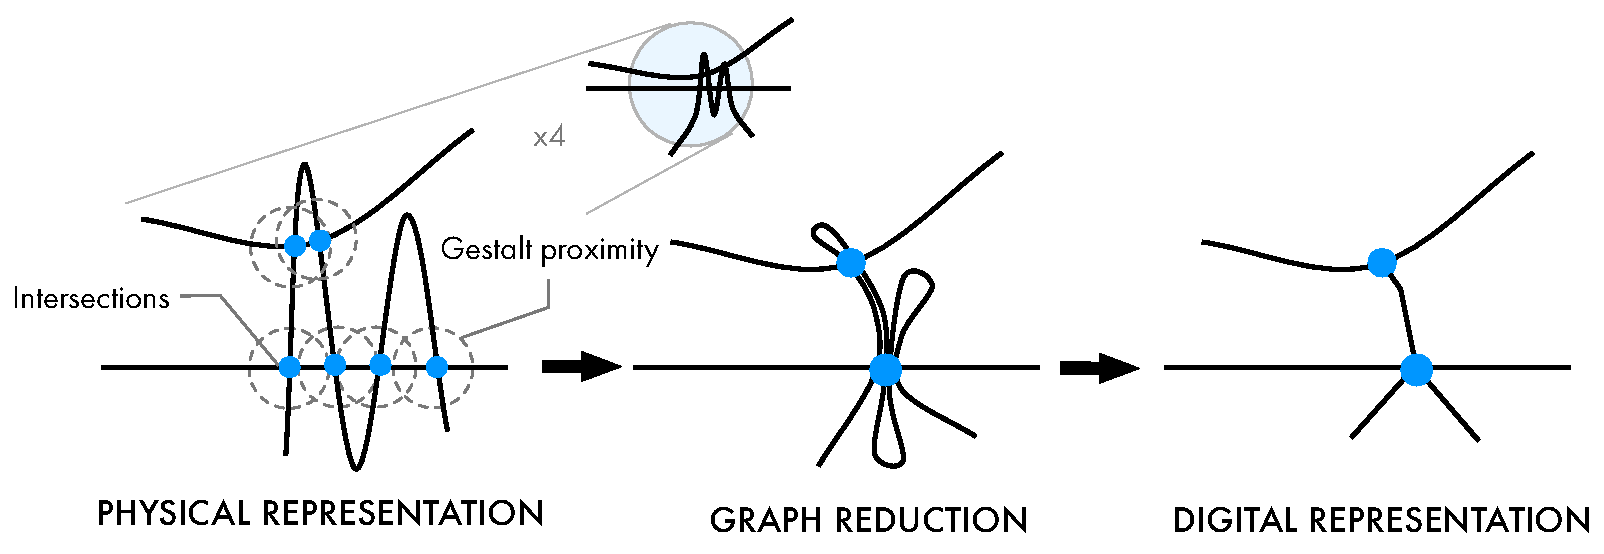
\includegraphics[width=1.0\columnwidth]{figures/gestalt.pdf}
        \caption{The complexity of a simple drawing, such as a scribble, adds significant computational complexity to a graph representation of a circuit. Ellustrate groups physically-close clusters of vertices together, reducing the complexity of the graph. }
        \label{fig:gestalt}
        \vspace{-16pt}
      \end{figure}

      \textit{Graph Extraction}.
      At the point when a user finishes drawing their Ellustrate circuit, we have an unconstrained number of SVG paths $p$. 
      Through a set of post-processing steps, we extract an undirected graph representation of the circuit as an adjacency list $\langle V, E \rangle$. However, because the direction of electric current takes the path of least resistance, we must first decompose intersecting paths.
    %   % (e.g. loops $\ell$, crosses)
    %   For each path intersection $s$ and self-intersection $t$, relevant paths are sliced at that intersection yielding $2(s + t)$ new paths. Intersections are disregarded if they occur at the start or end of the path, or if the two paths in question are collinear.
    %   For each blob intersection $b$, we draw a line from the blob center to the intersection point on the blob boundary yielding $b$ new paths.
    %   We then build an undirected $G$ using an adjacency list $\langle V, E \rangle$. We represent the start and end of each path as a vertex on the graph ($v = 4(s + t) + 2p + 2b $), and encode each vertex with its position on the canvas. An edge is defined as a connection where two vertices are collinear on a path or intersect another vertex; each edge is encoded with its material composition and cross-sectional area.
      % TOTAL VERTICES V = 4(s+t) + 2p + 2b
      % AFTER OPTIMIZATION V = s + t + b + 2p
    Let $t$ represent the number of path intersections, $s$ the number of self-intersections, and $b$ the number of blob intersections in an unprocessed design. For each path-intersection and self-intersection, we slice associated paths at their intersection point, yielding at least $2(s + t)$ new paths. Intersections are disregarded if they occur at the start or end of the path, or if the two paths in question are collinear. For each blob intersections $b$, we draw a new path from the associated intersection point on a blob boundary to the blob center, yielding $b$ new paths. 
    
    We then populate the adjacency matrix using the start and end of each path as a vertex, encoding each vertex with its position on the canvas. An edge is defined as a connection where two vertices are members of the same path or intersect with another vertex; each edge is encoded with its material composition and cross-sectional area.
     Dependent on  a user's drawing style, the adjacency matrix contains $|V| = 4(s + t) + 2p + 2b $ and an unconstrained $|E|$.
 
    \textit{Optimization step}. We uses the physical proximity of each vertex to simplify the graph. Vertices which are close together are joined as shown in Figure \ref{fig:gestalt}, while duplicate or self-referential edges are removed, reducing the total number of vertices by at least $3(s + t) + b$. This optimization reduces the number of vertices to $s + t + b + 2p$. To contextualize this information with respect to sketching, this optimization allows us to work with a 86 vertex graph of the octopus in Figure \ref{fig:teaser}a ($b$ = 32, $s$ = 9, $t$ = 17, $p$ = 14) compared to a 196 vertex graph.

      
    \textit{Calculating Path Resistance}. To provide a more accurate model of conductivity for each of these paths, we derive a model from a set of basic electronic rules. In order to determine the resistance of a path between to vertices on a the graph, we use breadth-first traversal to enumerate all paths.
    We collect the traveled edges into a set $Q$. 
    Each edge $e$ has previosly encoded associated material sheet resistivity $\rho_e$ and a sheet thickness $t_e$, which is simplified to sheet resistance\footnote{Sheet resistance $R_s$ is the measure of resistance of thin films with uniform thickness; conductivity is modeled as the ratio of cross-sectional area and the length of the path.} $R_s = \frac{\rho_e}{t_e}$.
    
    We derive the resistance $R$ of a set of edges $Q$ by traversing the edges and summing resistance as derived from cross-sectional area, which follows:
        \begin{equation}
            R =  \sum^{e \in Q} R_s \int_{i=0}^{n}  \frac{1}{w_i} dl
        \label{eq:resistance}
        \end{equation}
      where $n$ is the euclidean length of an edge, and $w_i$ is the width of the path at offset $i$. Under this model, a uniform line \SI{2}{\milli\metre} thick and \SI{20}{\milli\metre} in length made with silver ink ($R_s = 0.5$) has a resistance of \SI{5}{\ohm} whereas a similar mark made with conductive thread (W = \SI{15}{\micro\metre}, $R_s = 2400$) has a resistance of \SI{1.8}{\ohm}.

    \begin{figure}[t]
    \centering
    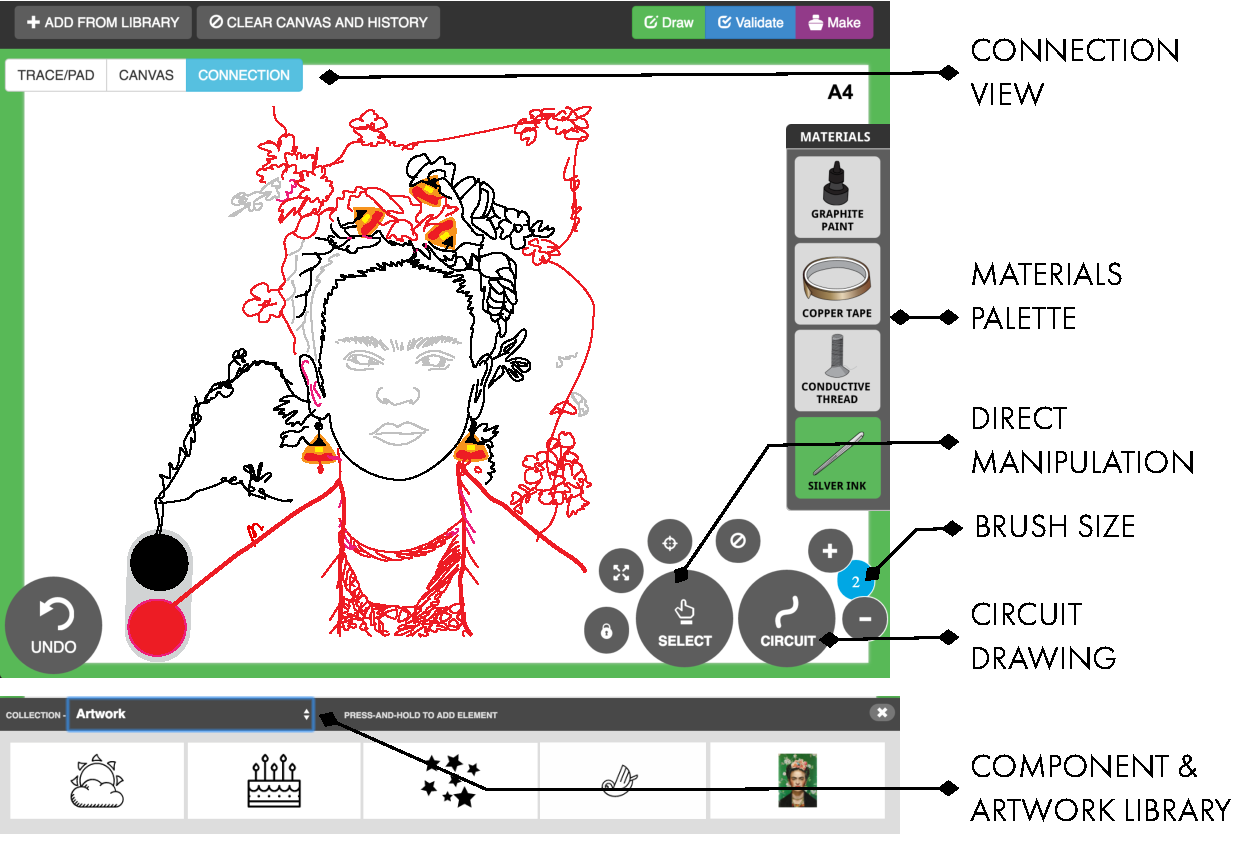
\includegraphics[width=1.0\columnwidth]{figures/designtool.pdf}
    \caption{Design step of Ellustrate, which allows a user to sketch a digital representation of a circuit prior to fabrication. The design tool features: connection point highlighting, direct manipulation tools for circuit elements, a tool for sketching traces, and a library of artwork and circuit component footprints.}
    \label{fig:design_tool}
    \vspace{-16pt}
    \end{figure}
    
\section{Digital Design Tool}
    In this section we detail common concerns of traditional circuit design, and how Ellustrate approaches these circuit constraints using simple visual rules.

    \subsubsection{Preventing shorts}
    Connections must have an adequate resistance to prevent electrical shorts. As such, paths that originate from the voltage source (\nt{PWR}) cannot make contact with paths connected to ground (\nt{GND}). As encoded within the SVG, we color-code paths, pads, and other conductive elements with respect to their polarity using conventional color schemes: red (positive), black (negative), or gray(neutral). To prevent shorts, we establish the following visual rule:
    \\
    \\
    \noindent\fbox{%
    \parbox{0.465\textwidth}{%
       \textbf{Visual Rule I.}
       Connections can only be made from/to similarly-colored (i.e. red\textbar red) elements or from/to neutral elements (i.e. gray).
        }%
    }
    \\
    \\
\begin{figure}[h]
\centering
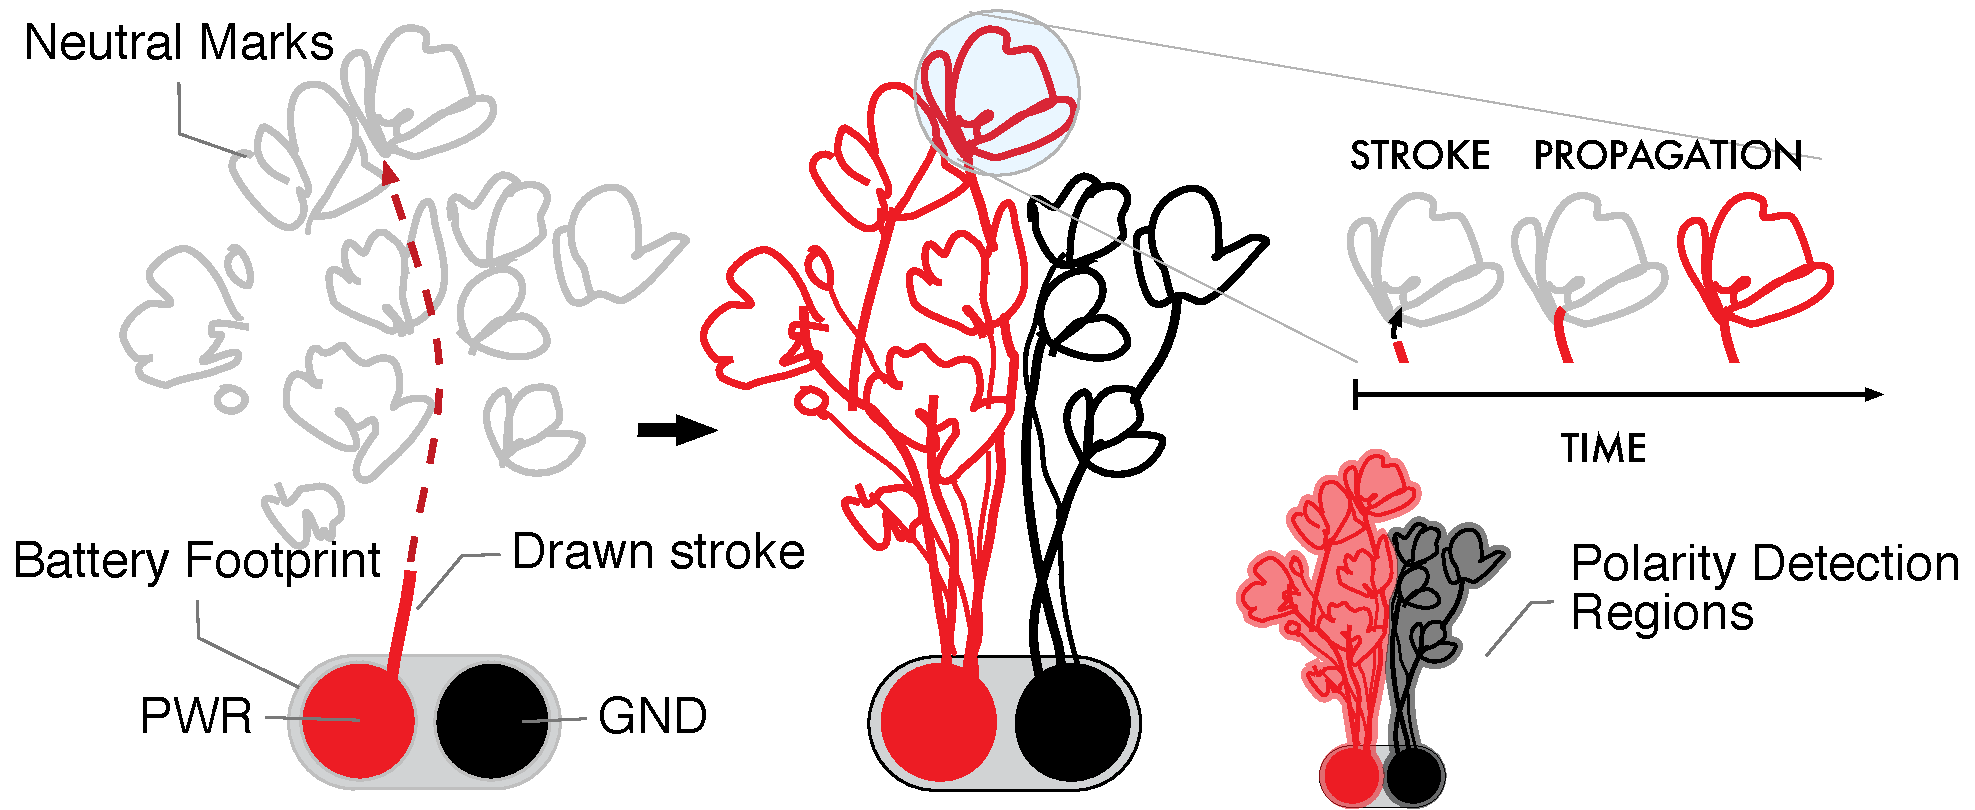
\includegraphics[width=1.0\columnwidth]{figures/propagation.pdf}
\caption{When a user's stroke intersects existing neutral conductive elements, the polarity of the stroke is propagated and coloring is updated. Polarity detection regions keep track of polar areas of the graph in real-time so as to detect shorts.}

\label{fig:propagation}
\end{figure}
    If a polar connection makes contact with a neutral element, the polarity is propagated to all elements touching the neutral element (Figure \ref{fig:propagation}). 
    Our tool validates this rule in real-time, ensuring that electrically-incompatible elements do not exist during draw-time, and is detailed in the following section. 

    \noindent\fbox{%
    \parbox{0.465\textwidth}{%
       \textbf{Visual Rule II.}
       All polar elements need to be connected to the respective battery pad.
        }%
    }
    \subsection{Legibility}
        In order to aid the user to parse the circuit from a visually complex design, we introduced two visual mechanisms: a) \textit{glow}, whenever an element is referenced by the tool, a ``glow" treatment is applied. Our treatment is a blue shadow with a large blur radius for validation, and a purple overlay for fabrication (Figure \ref{fig:fab_tool}); b) \textit{thinning}, although not an issue with thin-stroke mediums, some line weights (e.g., copper tape) occlude electrical connections. When triggering the connection view in Figure \ref{fig:design_tool}, design traces are thinned to hairline width and a visual marker is placed on all intersections of the design.
        
\subsection{Validation}
    Validation of the design is presented to the user during the design process and once the design has been completed. % This was mainly to minimize the intrusion the digital assistance coach. 
    \subsubsection{Real-time validation}
        To detect when users accidentally ``cross wires", we implemented real-time polarity collision detection by keeping a map of polar regions on the canvas (Figure \ref{fig:propagation}). This map is represented as a set of polygons constructed from the union of previously added conductive elements (in expanded form).
        If the user draws an electrically incompatible segment inside a polar region, a dialog modal alerts the user to the error, visually indicates and removes appropriate offending elements (Figure \ref{fig:process_flow}, center).
    \subsubsection{Post-design validation}
        We run a set of validation rules against the extracted circuit graph to provide users with feedback on the electrical validity and fabricatability of her or his design. 
            \begin{itemize}
                \item \factor{BATTERY CHECK}. Verify that a voltage source exists.
                \item \factor{CONNECTION CHECK}. For all LEDs, verify that there exists a path to ground and a path to power.
                \item \factor{POWER CHECK}. For each path from \code{PWR} to \code{GND}, extract the LEDs along the path. Sum the associated voltage-drops of each LED. Check that the voltage drop is not greater than the \code{PWR}.
                \item \factor{RESISTANCE CHECK}. For each path, verify that the resistance is below a threshold. 
                \item \factor{FAB CHECK}. For each path, verify against fabrication-specific constraints (e.g. a warning for long traces might cause a higher chance for fabrication error).
            \end{itemize}
        These checks produce error, warning, or success indicators in a validation side panel (Figure \ref{fig:process_flow}, center); selecting a validation error or warning highlights appropriate elements in the design. 
    
    \begin{figure}[t]
    \centering
    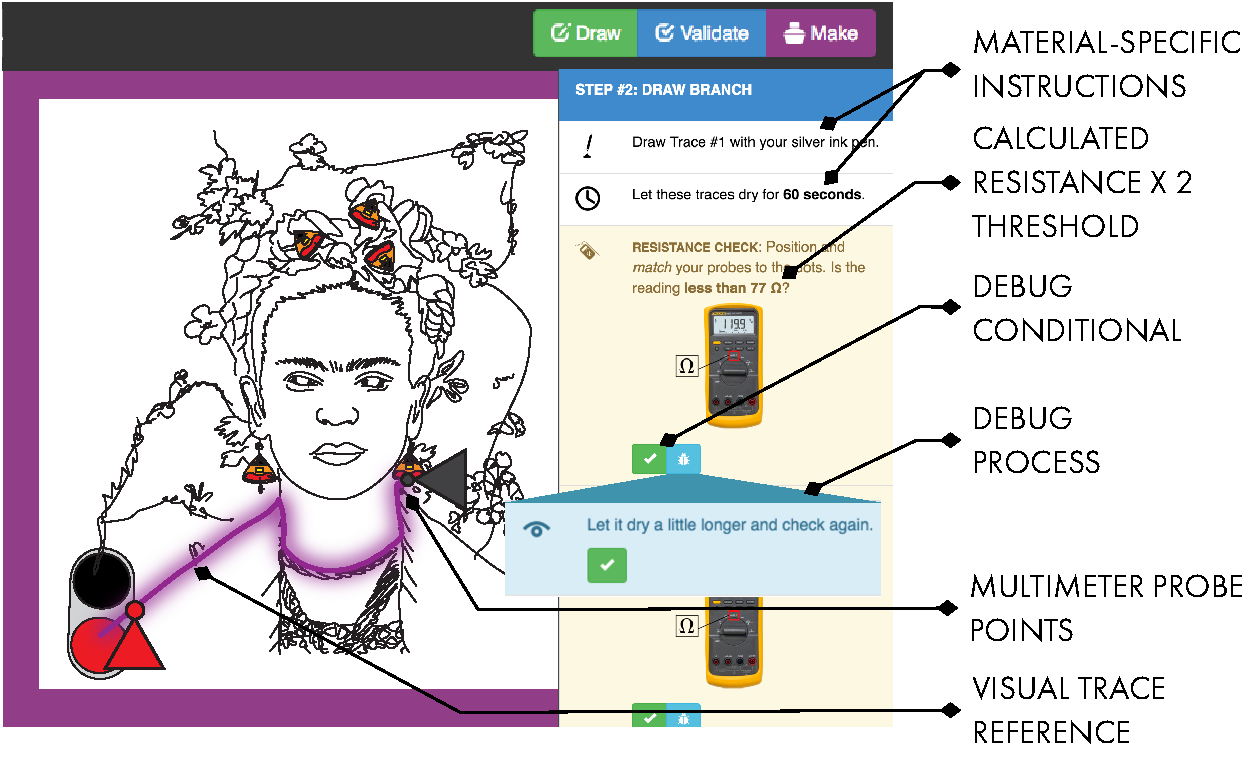
\includegraphics[width=1.0\columnwidth]{figures/fabtool.pdf}
    \caption{Fabrication phase of Ellustrate, produces design-specific instructions that decomposes a design into a modular fabrication routine. Visual markers indicate processes such as checking resistance. Conditional instructions allow for users to verify step, or receive debugging assistance.}
    \label{fig:fab_tool}
    \vspace{-16pt}
    \end{figure}
    
\section{Fabrication Tool}
    Once a circuit has passed digital validation, we provide a set of design-specific fabrication instructions and schematics. For clarity, we describe the fabrication system with respect to silver-ink as the conductive material, but detail which portions of this process was applied to other materials as well. 

    \subsection{Design schematics}
        The Ellustrate design tool outputs a to-scale version of the circuit as an SVG file, which is then printed or transfered onto a circuit substrate (e.g. paper, fabric, etc.). Conductive paths are denoted with dashed magenta lines to indicate where traces should be drawn, while each component footprint is outlined and labeled. Lastly, a printable bill-of-materials (BOM) is produced to aid with planning and record-keeping.
    \subsection{Design-specific fabrication instructions}
        To prevent common fabrication mistakes and to lay out an easy-to-debug circuit, Ellustrate generates instructions that encourage modular fabrication. To decompose the circuit graph, we query our scene graph for all LEDs on the canvas. We then extract the shortest (least resistant) path to power (\code{CVTB}) and to ground (\code{CGTB}) for each LED, and order these paths by length, which we term \textit{branches}. By fabricating each branch in sequence, a user can modularly test each branch in isolation. We arrived at the following fabrication procedure for circuit building through several pilot iterations with target users. For each instruction, our tool highlighted relevant parts of traces and components. For instructions that required the use of a multimeter (\code{MULT}), our tool displayed an image of the multimeter with the correct dial placement and visually-annotated where multimeter probes should be placed on the circuit (Figure \ref{fig:process_flow}, right). 

        Each instruction set begins drawing the initial traces originating from the power source with affixing a power source to the circuit. Since a power source is a common requirement for testing each branch, we keep it affixed throughout the procsss and reduce the number of variables if debugging is necessary.
        
        \noindent\fbox{%
            \parbox{0.465\textwidth}{%
                \begin{center}
                \textbf{\textit{Battery Instruction Set}}
                \end{center}
                \vspace{5pt}
                \begin{enumerate}
                      \item {[}Draw{]} the initial portion of all traces originating from the battery. [Dry].
                      \item Add the battery.
                      \item Power Check: For each power-ground path, check that a voltage of approximately 3 V is observed. (\code{MULT})
                \end{enumerate}
            }%
        }

        We then append steps for each branch to the instruction set. Certain steps require confirmation from the user to proceed, and, in the case of a negative confirmation, a debugging step is added to the instruction set and removed once resolved (Figure \ref{fig:fab_tool}). In addition, material-specific instructions are generated to aid with fabrication. For instance, in the case of silver-ink, drying time is affected by the amount of ink deposited by user and can vary from user to user. A drying time of 60 seconds is recommended (indicated by a countdown timer), which is long enough for most cases. Since wet ink has a higher resistance (which might impede circuit function), we also instruct users to test the trace resistance before proceeding. 
        %Utilizing our modeled conductivity, we can provide users an idea of what type of resistance they should expect, as well as a simple countdown timer to aid in determining the necessary time for the conductive ink to dry.
        
        \fbox{%
            \parbox{0.465\textwidth}{%
                \begin{center}
                \textbf{\textit{Branch Instruction Set}}
                \end{center}
                \vspace{5pt}
              \begin{enumerate}  
                  \item {[}Draw{]} both positive and negative traces in branch, [dry].
                  \item Check resistance of positive trace is about 2X [calculated resistance]. If not, [dry, widen, continuity]. (\code{MULT})
                  \item Check resistance of negative trace is about 2X [calculated resistance]. If not, [dry, widen, continuity]. (\code{MULT})
                  \item Place LED, pay attention to orientation; [handling].
                  \item Check if LED turns on. If not, [press down, go to step 2]
              \end{enumerate}
            }%
        }
        
        Similar instructions are substituted or added for using and debugging different materials, such as:
        \begin{itemize}   
          \item {[}Dry{]} Material-specific drying times (e.g. BareConductive graphite ink takes longer to dry than CircuitScribe silver ink). 
          \item {[}Widen{]} Thickening traces for higher resistance. 
          \item {[}Handling{]} For circuit stickers, ensuring that adhesive pads are ink-free, avoiding removing stickers from paper, not touching adhesive side. % Copper tarnishes from hand oils; wash your hands. 
          \item {[}Continuity{]} A continuity issue results when a trace is not fabricated correctly; a break in this trace will result in an interrupted connection preventing the flow of electricity. Use the multimeter in continuity mode and place both probes at [start]. Move one probe towards [end], checking that the trace is continuous (beep throughout).  
          % \item {[} Polarity Check {]} A user is provided with this template circuit which connects two traces to the a battery. A user can place the component of interest, such as an LED, and check the polarity of the component by placing it on the traces and observing changes in behavior. Should a user experience a non-working LED, they are encouraged to verify that the orientation of the LED be correct. Although we don't foresee these issues being of major concern since LEDs are housed in perceptually-identifiable packages, we recognize polarity being a common issue and provide a simple tool to address it.
          \item For conductive thread, larger patches need to be sewn for connection terminals; single strands may not be conductive enough. 
          \item For copper tape, a common debugging technique is to lay additional copper over problem areas. A rule of thumb is to use continuous pieces of tape. To reduce connection errors and make copper tape more aesthetic, one can use a bone knife to press-down, reduce tarnish, and smooth copper tape. 
        \end{itemize}

\section{EVALUATION}
    The goal of our formal user study was to conduct a usability evaluation of the tool, specifically observing how circuit design contraints influence the visual aesthetic and how fabrication assistance influences agency. 

\subsection{Participants}
    We recruited 10 participants (avg. 28 years, 7F, 3M) well-versed in visual design, but with no prior experience with circuit design. Proficiency was self-reported in a preliminary survey. Participants were recruited from a mailing list of Architecture, Art, and Design students at our institution and from the surrounding community via Craigslist.

\subsection{Materials}
    We constrained our evaluation to a single circuit building material --- silver ink was chosen due to it's user-friendly pen form factor that is a tangible analogous to the Apple Pencil. For the study, our electronics library was constrained to fixed set of finger-sized manipulatives: 5 Chibitronics LED stickers, and a single CR2032 coin-cell battery. We also exposed a set of SVG graphics shown in Figure \ref{fig:design_tool} with different layout compositions (figurative, linear, radial, and random placement) in order to evaluate how users navigate circuit rules with spatial constraints. 

\subsection{Study Design}
    Each participant was invited to individually meet with us in our studio space. Participants were paid \$20/hr; each session lasted two hours and consisted of a circuit and tool tutorial, a digital design task, a physical hand-fabrication task. We also conducted interviews before and after each session. Participants were also asked to share out-loud their reflections on tools and design process specifically vocalizing their design choices and shifts as they went through the workshop. 
    %Due to the visual complexity of the circuits, the experimenters aided with interface and fabrication issues when they arose. We report such occurrences for future work to support a larger corpus of visual styles.
    
    \begin{figure}[t]
    \centering
      \includegraphics[width=1\columnwidth]{figures/Ellustrate_figures_Users_in_action}
      \caption{During the formal user study, users a) sketched their circuit ideas with the design tool, b) fabricated the circuit, c) checked circuit validity using a multimeter and, d) debugged their circuits by pressing on components.}~\label{fig:users-in-action}
      \vspace{-20pt}
    \end{figure}

    % power requirements
    \textit{Warmup}. We provided participants with relevant background information for understanding the primary concerns of circuit design and building. A brief introduction covered basic electrical design rules (e.g. connecting power and ground, avoiding shorts) and operation of equipment (drawing traces with a silver ink pen; checking resistance and voltage with a multimeter). Tutorial material was available as reference throughout the study. 

    \textit{Design Task}. Participants were then given the task to design a circuit with five LEDs in parallel, with at least one background artwork incorporated for a period of 20 minutes. A five LED circuit provided a reasonable level of routing and creative challenge to be solved within 20 minutes. Parallel circuits also tend to create more routing complexity in an Aesthetic Circuit and require more creative solutions. If there were issues, they were asked to attempt to fix and iterate on their circuit design using features provided within the tool. 

    \textit{Fabrication Task}. Once successfully validated, our system produced fabrication instructions. A to-scale schematic was printed. Users were asked to fabricate their circuits using five circuit sticker LEDs. They were given 40 minutes to complete the task using fabrication and debugging instructions provided by the tool.  

    We asked participants to separately rate their experience with the design tool and the fabrication tool using five-point semantically anchored Likert questions (1=Strongly Disagree, 5=Strongly Agree):
    \begin{itemize}
      \item \factor{Assistance (As)}: The tool helped my circuit [designing/fabricating] process.
      \item \factor{Pre-Agency (pA)}: I feel capable of [designing/fabricating] a circuit before using the tool.
      \item \factor{Post-Agency with Tool (ApT)}: I feel capable of [designing/fabricating] future circuits with the tool.
      \item \factor{Post-Agency without Tool (Ap)}: I feel capable of [designing/fabricating] future circuits without the tool.
    \end{itemize}
    In particular, \factor{ApT} describes the experience of designing a circuit with Ellustrate, while \factor{Ap} generalizes to how Ellustrate may serve as a tool that enables lasting skills in Aesthetic Electronics design and fabrication.

\section{Results}
All participants successfully completed their designs; some designs are represented here in Figure \ref{fig:user-artwork}. 
We first report quantitative results and then discuss interview responses in the context of specific observations and insights from the study.

\begin{figure}[t]
\centering
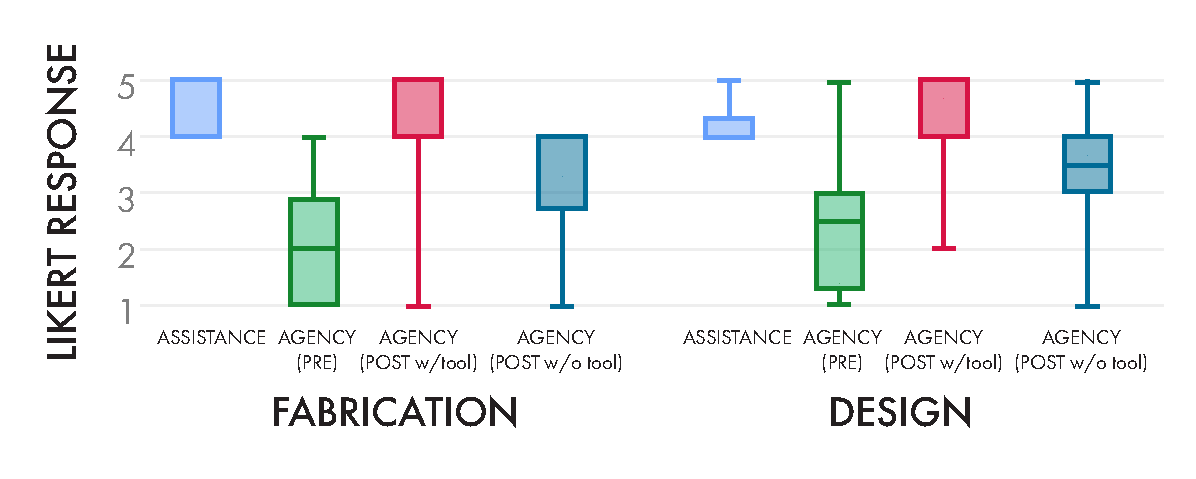
\includegraphics[width=1.0\columnwidth]{charts/boxplots_quant.pdf}
\caption{Tool evaluation responses. Overall, participants reported feeling more agency to create their own circuits after using Ellustrate, and felt that the tool assisted them with both design and fabrication.}
\label{fig:fab_tool_results}
\vspace{-20pt}
\end{figure}

Before using Ellustrate, users expressed uncertainty and apprehension when asked to design and fabricate an Aesthetic Circuit, respectively (design: \factor{pA} $2.4 \pm 1.26$, fabricate: \factor{pA} $2.1 \pm 1.2$). We were surprised to find that the mentioning of the word "circuit" elicited fear in some participatns. 
  \begin{myquote}
  \vspace{-2pt}
    \participant{Participant \#072}:
    \quoted{ I just want to make sure you know, I really, really don't know anything about circuits.}
    \vspace{-2pt}
  \end{myquote}

For both the design and fabrication tool, users felt that the tool has helped them on their design and fabircation processes (design: \factor{As} $4.2 \pm 0.42$, fabrication: \factor{A} $4.4 \pm 0.52$). After using the tool, users felt capable of designing and fabricating Aesthetic Circuits in the future with the aid of the design tool (design: \factor{ApT} $4.0 \pm 1.22$, fabrication: \factor{ApT} $4 \pm 1.7$), but slightly less capable of doing so without the aid of the tool (design: \factor{Ap} of $3.4 \pm 1.27$, fabrication: \factor{Ap} $3.3 \pm 1.3$). 
  
It was interesting to note that users with more visually complex designs that require multiple trial-and-error iterations to balance the visual design and electronic routing were more likely to report higher reliance in designing Aesthetic Circuits without the tool in the future (lower \factor{Ap}. In future work, we would like to investigate features that could further encourage users to create complex designs through iterations.
  
 \subsection{Design Classifications}

 We distinguished three types of marks that characterize how participants navigated around circuit rules to create their visual design, as detailed below:
  
  \begin{figure}[t]
\centering
  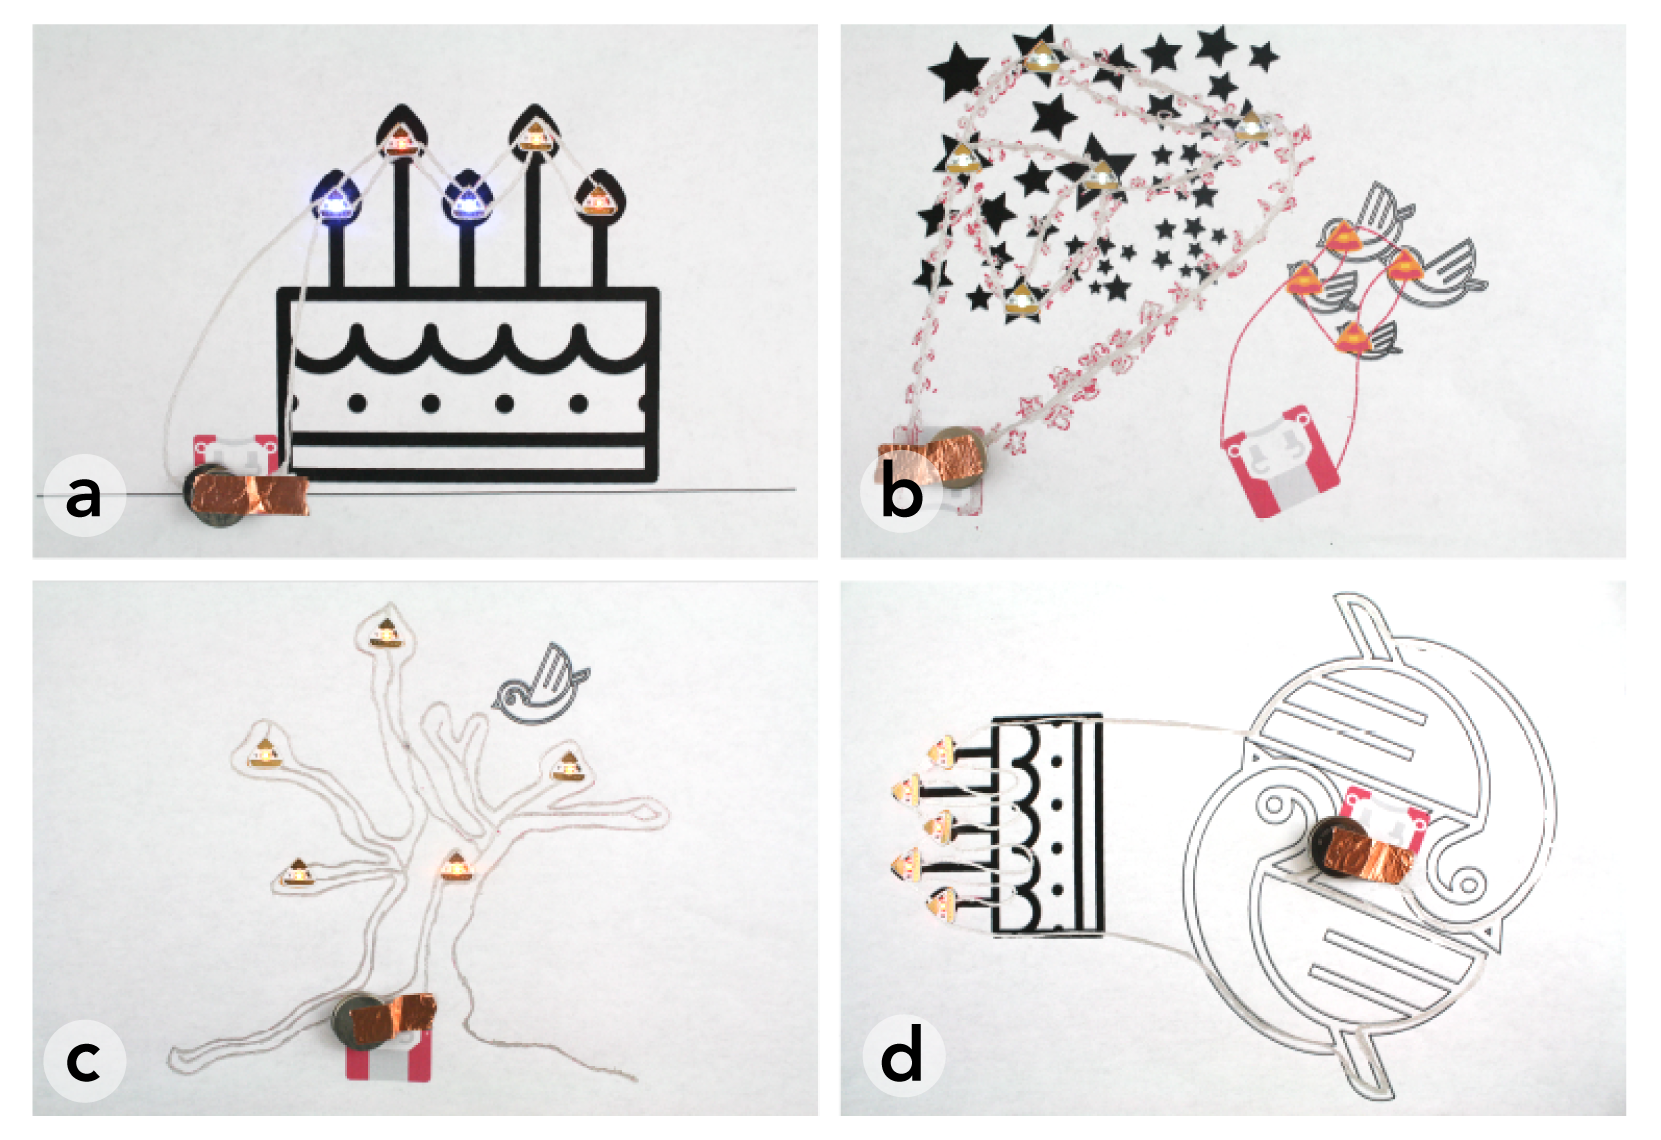
\includegraphics[width=1\columnwidth]{figures/users_final_des}
  \caption{Completed circuits from the user study drawn in silver ink on paper. Circuit designs show examples of a) functionalist, b) mimetic, c) constructive, and d) metaphorical marks.}~\label{fig:user-artwork}
  \vspace{-20pt}
\end{figure}

  \textbf{Functionalist:} While all participants tended to position LED footprints in semiotically relevant places (e.g. matching the triangular shape of the LED footprint with the candle flames, placing LEDs at the tips of the branches), some participants preferred a functionalist aesthetic, connecting electrical components using straight lines that minimized distance and distractors. Figure \ref{fig:user-artwork}a shows an example of a functionalist design. 

  \textbf{Mimetic:}
  Other designs adhered to the design language of the choosen SVG elements. An example of a mimetic design is shown in Figure \ref{fig:user-artwork}b, where the participant drew traces as a collection of twinkling lights, extended the visual texture of the background star field SVG.  In these scenarios, because participants mimic the existing design language, the choice of SVG highly influences the aesthetic of participants' final designs.
  
  \textbf{Constructive:} In contrast to functionalist and mimetic lines, some participants drew objects wholly outside of existing SVG scaffolding. Notably, Figure \ref{fig:user-artwork}c shows a circuit as a tree, where the user carefully interleaved electrically-opposite strokes to form the branches and roots; the SVG in this instance (a bird) is used solely to contextualize the tree. 
%   The additional stars emulates the existing texturing of the SVG.
  %Interestingly, the participant drew a graphic correspondence between then bird and tree branches, as well as a semantic correspondence with branching wire (a concept from electrical engineering) the tree branches.

  \begin{myquote}
  \vspace{-2pt}
    \participant{Participant \#156}:
    \quoted{I thought of something where I can branch out the wires, and I thought ``bird and branches.''}
    \vspace{-2pt}
  \end{myquote}
  
  \textbf{Symbolic:} Some participants went beyond using lines as a means of connecting wires, but instead as a mean of ascribing meaning to lines. Figure \ref{fig:user-artwork}d shows a ``yin-yang'' formed by two rotated bird forms. Traces and other footprints then conform to the meaning established by the birds. With metaphorical lines, participants satisfied not just two criteria: a) functional requirements of a trace in a circuit and b) aesthetic considerations, but also developed a ``language'' or a system of meaning based on the traces. We observed users use this ``language'' to tell a story with their circuit design, which was also observed in prior circuit sketching workshops~\cite{Jacoby:2013cq}.
  %This is semiotics, the emergence of artistic talent in a new circuit-drawing medium. 

  \begin{myquote}
   \vspace{-2pt}
    \participant{Participant \#499}:
    \quoted{The birds represent ying and yang, and the battery in the center represents the energy coming out of them ... the stars are tied together with twinkle light ropes, and the birds are flying towards the pretty lights.}
    \vspace{-2pt}
  \end{myquote}

\section{Observations and Insights}
In the following section, we report important insights derived from the user studies.

  \subsection{Translation Between Digital and Physcial Mental Models}
  We found that participants with no circuit experience relied heavily on the interface mechanisms used to convey circuit rules, adopting the visual vocabulary of the circuit design interface (e.g. ``red and black'' vs. ``positive and negative'').
  \begin{myquote}
   \vspace{-2pt}
    \participant{Participant \#499}:
    \quoted{I know there two silver traces can't cross - they are red and black and I need to be careful to not draw them too close to each other. }
    \vspace{-2pt}
  \end{myquote}
 Some users memorized the colors of the traces in their designs, and transferred that representation to their physical circuit fabrication. This observation shows opportunities in injecting more important circuit design concepts as visual representation, such as current as river water, within the digital design tool.
  

%  \subsection{Step-by-step Fabrication Can Overconstrain}
%  Although constraints are well-documented in HCI research to improve creative thinking, we found the constraint of an instruction set during the physical fabrication of participant circuits often inhibited participant's ability to develop a creative mental model for the circuit. The step-by-step or ``checklist'' style fabrication pipeline was the primary reason why users reported low agency (\factor{Ap, ApT}) after completing the task with the tool. In particular, participants who self-identified as artists found that the fabrication tool restricted their sense of creativity.
  % These participants reported a lower average \factor{AGENCY POST- (WITH TOOL)} of $1$, even though they reported an average \factor{AGENCY POST- (WITHOUT TOOL)} of $4$. When asked about what they disliked about the fabrication tool, both reported a reduced sense of agency in the artistic sense due to the constraints interface's pipeline.
%   \begin{myquote}
%   \vspace{-2pt}
%     \participant{Participant \#159}:
%     \quoted{There should be more options for shapes, and color as well as a grid. Validate mode is hard to get to... I kept forgetting to check the steps to complete them. It didn't exactly click for me.}
%     \vspace{-2pt}
%   \end{myquote}
%   These participants felt more empowered without the tool, wanted to generate their own methods of making versus fall into the regimen of the machine. \jasper{However, the artists didn't realize that they totally couldn't do anything without the tool} The underscores that pipeline processes did not adhere to creative thinking in the holistic design process.
%   While these participants reported feeling more empowered without the tool, we must also consider consider that the constraints of the step-by-step also allowed participants with less circuit knowledge to implement a creative designs without worrying about implementation details.

\subsection{Templating, Learning, and Improvising}
We were encouraged to find participants develops a sense of agency and early form of material and electronic fluency during the study sessions. When first started fabricating the circuits, participants find comfort and safety in the step-by-step fabrication guide. The format of a list, with additional debugging tips as an expandable-list feature, were particularly appreciated. 
  \begin{myquote}
  \vspace{-2pt}
    \participant{Participant \#081}:
    \quoted{I like that the list of steps is very clear, and the debugging tips are tucked away until you indicate that you have a circuit problem.}
    \vspace{-2pt}
  \end{myquote}
However, as they progress through the process, some find the format too rigid and wish to learn more about the rationale behind the guided steps. 

  \begin{myquote}
  \vspace{-2pt}
    \participant{Participant \#554}:
    \quoted{There is obviously some rules behind where to put the multimeter probes to debug, I would like the tool to explain that to me so that I can do it by myself.}
    \vspace{-2pt}
  \end{myquote}
  
  Some participants improvised new ways to fabricate and debug by relying on their own intuitions in order to bypass a certain step within the guide. For example, most users dislike waiting 60 seconds for the silver ink to dry the most, so some started blowing on the ink to get it to dry faster and move the paper around to see if there is a color difference between dry and wet ink. In-depth learning and improving occurred at different point of the process for each participant. We were encouraged by the diversity of learning styles and the early development of fluency, and we see this as an opportunity to create more customizable instructions and learning materials for users in the future. 

  
%   \subsection{Incentivizing Tinkering and Debugging}
%   Because the step by step instructions created a guaranteed safety net, several users began to disregard the steps provided by the interface. Instead, once gaining proficiency and confidence with the tool and process, they began to make design decisions based off of their own intuition and developed their own behaviors independent of the step-by-step instructions, such as blowing on wet conductive ink to reduce drying times. Many sought to optimize and build on the fabrication process, commenting that allotted waiting time of 60 seconds was wrong and that they knew what was best after having debugged several traces.
%   % Also users had to learn to place the probes correctly, often the probe tip went into the paper
%   The conductive ink pen itself is something that users had to tinker with. Almost all users made their traces too small in the beginning, and then went back and widened their traces later as they saw fit. Because users were prompted to debug each trace during the step-by-step instructions, they had the opportunity to try new ways of drawing traces, and thus were able to adapt their cognitive model to the pen.
% %   They knew they could experiment with the pen and thus switched over from learning from the interface into learning from their own craft. This is tacit learning.
% %   Another type of behavior was \textit{forethought}, where users anticipated future issues with their design and adapted accordingly, disobeying the interface as necessary. Many participants learned to extended trace past the LED footprints, thinking ahead of how they would later need the extended portion to continue the trace in the next step.
%   In general, participants moved from wanting to plan everything out in the beginning, to wanting to be able to tinker and tweak their designs as they went along. Even thought step-by-step instructions might reduce creative agency, they introduce a favorable iterative design process that distinguishes coarse and fine-grain. \cesar{what is grained?} \ep{this paragraph is a bit long and wondering...tighten this up and get to teh point more quickly}
  
% %   \begin{myquote}
% %   \vspace{-2pt}
% %     \participant{Participant \#857}:
% %     \quoted{Maybe have more explanation of why the circuit should be the way it is--more details to understand why something went wrong.}
% %     \vspace{-2pt}
% %   \end{myquote}
  
%  The tension that results from these inconsitencies between the tool and the phyiscal circuit motivated participates to incorporate debugging into their cognitive models and find ways of debugging that work for them. Though, many participates expressed interest in the behind-the-scenes theoretical explanation of their designs. For example, participants often did not know how to react to negative voltage readings.
  
%   \begin{myquote}
%   \vspace{-2pt}
%     \participant{Participant \#81}:
%     \quoted{The multimeter reading is in megaohms instead of ohms, and the voltage is negative. That seems to be okay in this case, but why? Which numbers are okay?}
%     \vspace{-2pt}
%   \end{myquote}
  

%   \begin{myquote}
%   \vspace{-2pt}
%     \participant{Participant \#554}:
%     \quoted{It'd be much more satisfying if you have contextual knowledge, it'd enable you to become more creative}
%     \vspace{-2pt}
%   \end{myquote}
  
%   Here we see that designers are motivated to learn circuit theory because they seek to improve their debugging skills with their own design. In addition, future circuit design interfaces may benefit from additional educational elements that teach users circuit concepts beyond those required to complete their designs.
  
%   \begin{myquote}
%   \vspace{-2pt}
%     \participant{Participant \#449}:
%     \quoted{I was thinking of moving the black around, but it looks like the black is completely enclosed... Okay, well now... Drastic changes to the plan...}
%     \vspace{-2pt}
%   \end{myquote}
  
%   However, the drive to tinker and recraft their designs became apparent later on. This was ideal as it allowed users to experientally naviagate the tension between aesthetical and electrical considerations.
  
%   \begin{myquote}
%   \vspace{-2pt}
%     \participant{Participant \#554}:
%     \quoted{Ideally, it would be more useful to fundamentally understand the concept, then I can figure out the steps on my own.}
%     \vspace{-2pt}
%   \end{myquote}
  
%   \subsection{Sandboxing}
%     For many, their initial designs were just exploration of the constraints, many, althought they could modify their designs a little bit to adjust to the red and black constrains (e.g. 449), many felt the need to start from scratch after they learned about the domain.
    
%     In the initial stages, users based everything around a plan. In the design step, they thought of their circuit in terms of a plan and were able to abstract away many non-essential practical considerations, and this proved useful for enabling participants to quickly develop a prototype without worrying about the implementation details.

\section{Limitations}
While we have highlighted the contributions of Ellustrate to the development of Aesthetic Circuits, there are several limitations to the current state of the design tool. 

\subsection{Electronic and Material Library}
We chose to focus on including several basic electronic and materials in our currently. We included Chibitronics CircuitStickers and LED's of various packages in the electronic library, and silver ink, grahite ink, and copper tape in the material libary. These components and materials were chosen because they were commonly used in circuit craft making, but they do not come close to being an exhaustive list of the electronics that can be used in an Aesthetic Circuits. If Ellustrate can successfully promote a literacy in creating Aesthetic Electronics, we imagine the library would have to greatly expand. The footprint of a wide variety of interactive electronics, such as pressure sensors, microphones, IR sensors, could be included. Moreover, some physical electronics that can be created directly with conductive painting, such as capacitors, paper speakers, and strain gauges, could be included in the library as well (where their electronic properties can be simluated dynamically with the design). 
\subsection{Circuit Drawing Capability}
The circuit drawing capability of Ellustrate could be improved on both the aesthetic drawing and circuit simulation front. Currently, the digital form factor, although more fluid than expected, left much to be desired from pen and paper, citing resolution and accidental markings (from digital artifacts). The number of drawing features within the tool was also significant fewer than visual designers are used to having. Circuit decomposition also faces unqiue problems as Aesthetic Circuits often contains a high number of trace intersections that are common in a paint-brush like drawing action. Ellustrate currently has difficulty validating circuits that contain a high number of intersections, which limits the copmlexity of artwork taht could be created with the program. 

\section {Discussion and Future Work}
Beyond the design and fabrication of Aesthetic Circuits, we envision Ellustrate to initiate in a broader conversation of the enablement of Aesthetic Electronics.


% \ep{you also really made a strong poush for aesthetic but didn't go deeply into this term and its usage...you coudl add mroe discussion on that (but likely much earlier in paper when you intruduce the term Aesthetic Electronics}
\subsection{Material properties for design}
Technological fluency, defined as ``the ability to understand, use, and assess technology beyond its rote application'', is seen as one of the fundamental quality that affords creativity~\cite{Lukens:2011jl}. As the landscape of interaction designs broaden to include a wide range of materials, including living cells in BioLogic, thermoplastic in ShrinkyCircuits, and polymer and air in Pneuduino, a fluency in material properties becomes increasing important in creating innovative tangible interactive platforms. Ellustrate aims to play a role in promoting the exploration of fundamental material properties by providing a digital platform for users to alter the electrical and visual properties of conductive materials - something most commonly thought of as digital in function (i.e. connected vs. not connected) by non-experts. Within Ellustrate, we have shown how users can explore the change in resistance and visual aesthetics as they widen and lengthen conductive traces or change the material used. Beyond understanding the nature of conductive materials, we hope to start a design conversation by disrupting the perception of an object that is well-defined - an electrical connection does not necessary take on the shape of a wire, but it could be made with something that has many variables that can be manipulated. We believe that Ellustrate could be used as a tool to democratize the critical thinking about materials, enabling the exploration of the next creative tangible interface. 
% \cesar{awesome about wire}


% \subsection{Resistance as a site for design}
%     There are several implications that arise from this model for path design: 1) branching non-connecting elements of the main trace are negligible since current does not travel through them giving users the creative freedom to be able to freeform traces without the risk of it effecting the circuit, 2) common circuit problems of having to resistive a trace and be alleviated by widening the trace either by thickening the area around the path trace or using connected branches.
\subsection{Online Community}
Ellustrate could have great impact on the hardware sketching practice as we develop an online community for users. Users could submit their designs and fabricated circuits to a share with the community. Moreoever, the community could contribute the fabrication and debug process, as well as tips and questions tagging specific steps. The framework of the digital tool - design, fabricate, and debug - accompanied with electronic properties analysis that are usually invisible to users could be expanded to include other Aesthetic Electronic input and output elements that are common to interaction design (i.e. capacitive sensors, strain gauges) as well. We envision the Ellustrate community to be capable of supporting users with richly diverse aesthetic styles, electronic experiences, and learning and teaching styles .

\section {Conclusion}
In this paper, we presented Ellustrate, a digital tool for designing and fabrication Aesthetic Circuits. We demonstrated its capability to assist in creating Aesthetic Circuits with different conductive and non-conductive materials - silver pen, graphite paint, conductive thread, fabric, and paper. We detailed algorithms specially designed to decompose and analyze Aesthetic Circuits, capable of extract electrical relevent traces for circuit analysis. Ellustrate was designed based on formative interviews of experts and pilot studies with visual designers in order to address common challenges Aesthetic Circuit designs. We also performed formal user studies to evaluate the designs and fabrication enabled by the design tool. Ellustrate (is rainbow and unicorn...)

\balance

\bibliographystyle{acm-sigchi}
\bibliography{ellustrate}

\end{document}
           %   \paragraph{The Water Metaphor}These are important design considerations for circuits. Mention the tried-and-true metaphors of current as water.
            %     \subsubsection{Visual Design Objectives}
            %     These are important design objectives that we wish to address with our study design. Things should be pretty.

        %      Circuit templates
        % Template circuits are well-known valid circuits with known acceptable resistance values and current readings. Unlike other work that incorporates a widget drag-and-drop interaction, we expose users to the actual circuit design. We dynamically map the circuit as it is constructed to have correspondence with the template circuit.
        % The mapping is done as follows.


        % Our templates currently include 3 and 5 LED parallelized circuits. *add information about series circuits and more variation in LED numbers. add information about battery holder and paper “pockets” and paper switches.*
